\chapter{Data analysis}
\label{chap:DataAnalysis}
\section{Data description}
Flight ticket prices were collected 4~times per day for a period ranging from the $9^{th}$ of July till the $29^{th}$ of September. During this data collection phase, airfares on the 22~routes described in \autoref{app:SelectedRoutes} were gathered on flights departing from the $20^{th}$ of August till the $30^{th}$ of September. In these 12~weeks, 158,553~files were requested from Google~Flights' RPC-servers, which resulted in a set of almost 18~gigabites of JSON~data. 15~of these requests failed at the first try, and had to be downloaded again one quarter of an hour later. Of these retries, the automated script also failed to download 2~files at the second request. These failures were the request made on the $20^{th}$ of September at 00:00 GMT+2 for flights departing from JFK to LHR on the $25^{th}$ of September and the request made on the $26^{th}$ of July at 00:00 GMT+2 for flights departing from LHR to LAX on the $1^{st}$ of July. As the next paragraphs will explain, these two~failures did not create any gaps of missing data in the final data structure.

After retrieval of the data all the JSON-files were parsed for single-legged return flights and categorized by outbound/inbound airport, and operating carrier. Each flight was distinguished using the characteristics described in \autoref{subsec:FlightTicket}, and departure times were converted to UTC\@. Next, the timeslot $p_{t_n}$ of the lookup time relative to the actual departure time was determined for each flight, where $n = \lfloor \frac{\scriptstyle{hours\ before\ departure}}{6} \rfloor + 1$. Because files were downloaded for 4~times per day, they can be assigned to timeslots consisting of 6~hours. For example, an airfare retrieved 33 hours before departure of the flight will be assigned to timeslot $p_{t_6}$, where $6 = \lfloor \frac{33}{6} \rfloor + 1$. Because ticket prices were acquired from 1~day up until 42~days before departure, a total of 168~timeslots are available ranging from $p_{t_5}$ till $p_{t_{172}}$.

After parsing of the files, the prices of the 6~hour timeslots were converted to represent daily values. To do so, every 4~timeslots where thus aggregated into a single airfare by averaging the values. For instance, the timeslots $p_{t_{17}}$, $p_{t_{18}}$, $p_{t_{19}}$ and $p_{t_{20}}$ were averaged into a single value $p_{d_4}$ representing the ticket price for that specific flight as available 4~days before departure.

\noindent
An illustration of this process is given in \autoref{fig:conversionOfTimeslotsIntoDailyAirfares}.

\begin{figure}
$$
\kbordermatrix{
           &\multispan4\hfill$\scriptstyle 1\,dbd$\hfill    &        \\
    \omit  &\multispan4\quad\downbracefill\quad             &        \\
    \#1    & p_{t_5} & p_{t_6} & p_{t_7} & p_{t_8} & \vrule & \cdots \\
    \#2    & p_{t_5} & p_{t_6} & p_{t_7} & p_{t_8} & \vrule & \cdots \\
    \vdots & \vdots  & \vdots  & \vdots  & \vdots  & \vrule & \ddots \\
    \#n    & p_{t_5} & p_{t_6} & p_{t_7} & p_{t_8} & \vrule & \cdots 
}
\Rightarrow
\kbordermatrix{
           & 1\,\scriptstyle{dbd}       & \cdots & 42\,\scriptstyle{dbd}              \\
    \#1    & \overline{p_{t_{5,6,7,8}}} & \cdots & \overline{p_{t_{169,170,171,172}}} \\
    \#2    & \overline{p_{t_{5,6,7,8}}} & \cdots & \overline{p_{t_{169,170,171,172}}} \\
    \vdots & \vdots                     & \ddots & \vdots                             \\
    \#n    & \overline{p_{t_{5,6,7,8}}} & \cdots & \overline{p_{t_{169,170,171,172}}}
}
$$
\caption{Conversion of timeslots into daily airfares}
\label{fig:conversionOfTimeslotsIntoDailyAirfares}
\end{figure}

When certain timeslots contain no price observation, this single timeslot is left out of the calculation of the average airfare for that specific number of days before departure. Only when all 4~of the timeslots for a specific day have no data available, the value in the new data matrix is assigned as \emph{missing value} (i.e., n/a). Due to this methodology in which the daily 4~data~points are aggregated into a single value, the 2~failures described earlier do not create any gaps of missing values in the final data matrix. \todo{analysis}

The conversion into daily values resulted in a database containing 462,662 unique flights which included 12,865,953 airfare observations. Due to Google Flights' nature of returning a limited set of airfares for each request, some flights did contain gaps of missing values within their data. In alignment with the study by \citeA{groves2013agent}, this paper therefore excludes flights for which less than $\frac{2}{3}$ of the possible airfare observations are available. So, because there are a total of 42~observations days prior to each flight, tickets that do have fewer points than $42 \times \frac{2}{3} = 28$ available will be excluded from the analysis. Next, because airlines are known to open and close specific price-buckets \cite{mcgill1999revenue}, some gaps were still present in the dataset. These gaps were filled with the data available from observations made in the future. For example, when a particular flight misses a price observation at 35~days before departure, but it does contain the airfare for 34 and 36~days prior to departure, the 35~days' slot would be filled with the same value as the 34~days before departure. In reality this would mean that when a customer's option expires, but the ticket is not available on the date of maturity (i.e., no price observation). The customer thus would have to wait till the airline resumes the sale of that flight. He would therefore get the ticket at the price in the future.

Missing data at for the last (few) days prior to departure are considered to be the sell-out of a flight. Because Google Flight's also offers Business and First class tickets, this implies that all the seats are completely sold out, and there is no possibility of still buying the ticket. This means that when a customer's option expires on such a ticket and he wishes to exercise it, an alternative flight has to be offered. To prevent such situations from happening, these missing data on sold-out flights is filled with a penalty similar to the technique used by \citeA{etzioni03}. By introducing such a penalty, the option valuation model is triggered into trying not to offer options when the probability of sell-out is high. Instead of the \$300,000 proposed by the authors, I have chosen to set the penalty at 3 times the average airfare at 1~day before departure. This is more realistic in a sense that the customer could be offered an alternative flight that leaves on the same day plus some extra form of monetary compensation. Furthermore this lower fill-value prevents penalties from biasing the airfares closer to departure.

An illustration of this data filling process is given in \autoref{fig:dataFillingOfMissingValues}. Airfares are given as integers representing the price in cents. As can be seen in the figure, the n/a-gaps are filled with the nearest available future price closer to departure. Furthermore, the missing value for the flight with id~\#3 at 1~day before departure is seen as a sold-out ticket. This value is filled with $3 \times \bar{c_1}$, where $\bar{c_1}$ represents the average of the airfares observed at a single day before departure.

\begin{figure}
$$
\kbordermatrix{
           & 1\,\scriptstyle{dbd} & 2\,\scriptstyle{dbd} & 3\,\scriptstyle{dbd}  & \cdots \\
    \#1    & 10000                & 12000                & 12000                 & \cdots \\
    \#2    & 20000                & \mathrm{n/a}         & 22000                 & \cdots \\
    \#3    & \mathrm{n/a}         & 32000                & \mathrm{n/a}          & \cdots \\
    \vdots & \vdots               & \vdots               & \vdots                & \ddots
}
\Rightarrow
\kbordermatrix{
           & 1\,\scriptstyle{dbd} & 2\,\scriptstyle{dbd} & 3\,\scriptstyle{dbd}  & \cdots \\
    \#1    & 10000                & 12000                & 12000                 & \cdots \\
    \#2    & 20000                & 20000                & 22000                 & \cdots \\
    \#3    & 3 \cdot \bar{c_1}    & 32000                & 32000                 & \cdots \\
    \vdots & \vdots               & \vdots               & \vdots                & \ddots
}
$$
\caption{Data filling of missing values (i.e., n/a)}
\label{fig:dataFillingOfMissingValues}
\end{figure}

The empirical dataset shows that in total 159,600 flights are not offered (i.e., sold-out) at 1~day before departure. These tickets take into account almost 35 percent of the all the flights available. Real-world data on the number of sold-out flights is very hard to acquire, because this value could give sensitive information on the performance of an airline.  \todo{Kindervater?}


After cleaning the dataset, it was split into two separate parts. The database used in this research contains airfare observations of flights departing in the period $20^{th}$ of August till the $30^{th}$ of September. As explained in \autoref{chap:Methodology}, the first 4~weeks of these departing flights --- $20^{th}$ of August till the $16^{th}$ of September --- will be used as the training set for the research. The latter 2~weeks --- from the $17^{th}$ of September till the $30^{th}$ of September --- will be used for testing the proposed option valuation models. This split resulted in a training set containing 321,545 flights, and a test set which includes 141,117 flights. An example extract of the final test data matrix used for the flights from AMS to JFK can be found in \autoref{fig:extractFromAMStoJFK}. In this extract, flight with id~\#4 was sold-out 1~day before departure, and that field was thus filled with $3 \times$ the average ticket price at 1~day before departure.

\begin{figure}
$$
\kbordermatrix{
           & 1\,dbd & 2\,dbd & 3\,dbd & 4\,dbd & 5\,dbd & \ldots & 42\,dbd \\
    \#1    & 57469  & 68619  & 122469 & 222469 & 109644 & \ldots & 65853   \\
    \#2    & 87119  & 87369  & 93019  & 84469  & 79469  & \ldots & 65853   \\
    \#3    & 87494  & 86694  & 94744  & 74569  & 70244  & \ldots & 65853   \\
    \#4    & 410951 & 134430 & 242480 & 108934 & 126369 & \ldots & 123357  \\
    \vdots & \vdots & \vdots & \vdots & \vdots & \vdots & \ddots & \vdots  \\
    \#252  & 68984  & 69094  & 64669  & 73219  & 70244  & \ldots & 65857
}
$$
\caption{Sample extract from test data matrix AMS to JFK}
\label{fig:extractFromAMStoJFK}
\end{figure}

\noindent
A further analysis of these datasets, including more specific statistical numbers on the 22~routes, can be found in \todo{table ref}

\todo[Table]{table with analysis of sets}


\section{Simulation model}

\subsection{Parameters of the simulation model}
As stated in the previous section, when calculating the customer's WTP and the seller's WTA, some parameters come to play. This section will elaborate on the precise implementation of these configurable options.


\paragraph{Option's number of days to maturity}
The parameter describing the number of days to maturity is directly related to the airfare~lock-in product itself. This property can be construed as the extra decision time a customer will gain from purchasing the option and gives the passenger the opportunity to wait a specific number of days $m$ without risking a fare fluctuation. This simulation will examine the effects on relative profits of offering options with 3, 7 and 14~days to maturity.

\todo{expectations?}

\paragraph{Passenger's arrival rate}
As described in previous section, this simulation will generate passengers to determine the performance of each model and configuration of parameters. A passenger will arrive at every day before the departure of the flight for the full observed 42~days. The number of customer arrivals is thus fixed per simulation and can be expressed as $42 - m$, where $m$ is the number of days to maturity.

\paragraph{Passenger's risk-utility}
In a risk neutral setting with shared information between seller and buyer, there would be no possibility of expected profits for the option writer. This is because the customer's Willingness To Pay will never exceed the Willingness To Accept of the seller. However, customers tend to be risk averse, and are therefore willing to pay something extra in order to prevent risk \todo[(ref)]{literature}. This means that these risk averse customers agree to pay for a premium on top of the current price of a ticket to fixate the price. The concept of such a risk premium thus allows for expected profits in a situation of equal information.

In this thesis, the level of risk aversion is simulated using the exponential risk-utility function for costs:
$$
u(p_t) = -e^{p_t/R},\hspace{2em}\text{where } R > 0
$$

The parameter $R$ is the level of risk aversion of a subject, which will approach risk neutrality as $R \rightarrow \infty$. The precise value of parameter $R$ is calculated using a certain risk premium $RP$. This premium is a percentage of the current price which the customer is willing to pay extra to buy off the risk. Because the parameter $R$ is influenced by different distributions of expected prices, this research will compute the value by considering a hypothetical situation: the customer will have the same utility for a fixed fare increased by $RP$ as for a variable price that has a 50\% probability of dropping half its value and a 50\% probability of increasing with half its value. This can be expressed using the following equation: 

\begin{align*}
    (1 + RP) \times p_t &= u^{-1}(0.5 \times u(0.5 \times p_t) + 0.5 \times u(1.5 \times p_t)) \\
    u^{-1}(x) &= R \log(-x)
\end{align*}

As an example, consider that the current ticket price is \$\,250, and the customer has a $RP$ of 10\%. Instead of buying the ticket immediately, the passenger wishes to wait till a later moment in time. He knows that the fare will not be stable, but will either have a 50\% probability of dropping to \$\,125, or a 50\% change of increasing to \$\,375. A risk neutral customer is not willing to pay anything for an option that fixates the fare at \$\,250, because $.5 \times 125 + .5 * 375 = 250$. However, the customer in this hypothetical setting is not risk neutral, but rather risk averse. As stated before, he is willing to pay a $RP$ of 10\% extra to fixate the price at \$\,250 instead of running the risk of a price increase:

$$
(1 + 0.10) \times 250 = 0.5 \times u(0.5 \times 250) + 0.5 \times u(1.5 \times 250)
$$

In which $R$ will thus have the value of 305, which leads to the risk-utility function of this specific customer of
$$ u(p_t) = -e^{p_t/305} $$

The function is also represented in \autoref{fig:RiskUtilityFunctionOfPassenger}. In this figure, one can see that the passenger's utility for a fixed price of \$\,250 is
$$ -e^{250/305} = -2.27$$

However, because of the uncertainties of price changes in the future airfare, the customer's utility in the hypothetical setting is
$$0.5 \times e^{125/305}+0.5 \times e^{375/305} = -2.46$$

This utility corresponds to a value of \$\,275, or 10\% risk premium on top of the current price. The increased price the passenger is willing to pay thereby thus implies the risk neutrality of the passenger.

\begin{figure*}
	\centering
	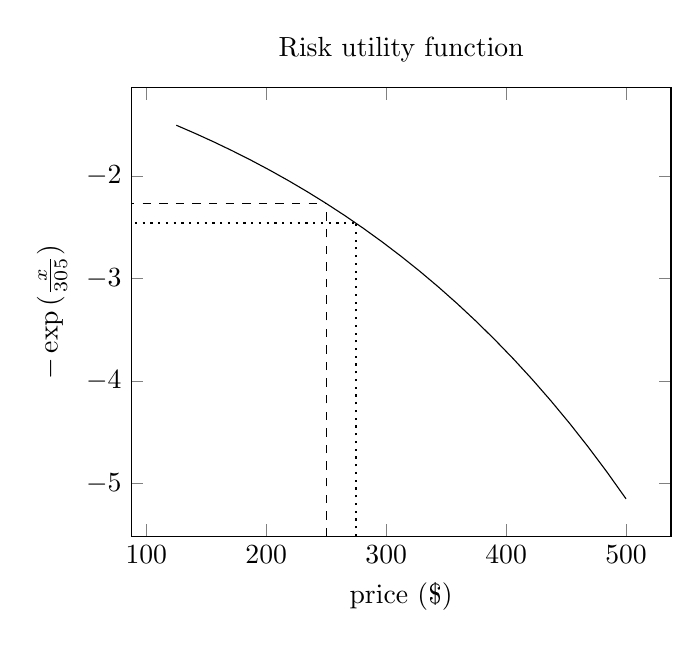
\begin{tikzpicture}[domain=125:500]
        \begin{axis}[xlabel=price (\$), ylabel=$-\exp{(\frac{x}{305})}$, title=Risk utility function]
            \addplot[mark=none] {-exp(x/(1.22*250)}; 
            %\addlegendentry{$-e^{(\frac{x}{1.22*250})}$}
            \draw[dashed] (axis cs:250,\pgfkeysvalueof{/pgfplots/ymin}) -- (axis cs:250,-2.27);
            \draw[dashed] (axis cs:0,-2.27) -- (axis cs:250,-2.27);
            \draw[dotted,thick] (axis cs:275,\pgfkeysvalueof{/pgfplots/ymin}) -- (axis cs:275,-2.46);
            \draw[dotted,thick] (axis cs:0,-2.46) -- (axis cs:275,-2.46);
		\end{axis}
	\end{tikzpicture}
	\caption{Risk-utility function of passenger}
    \label{fig:RiskUtilityFunctionOfPassenger}
\end{figure*}

After determining the risk-utility function of a passenger, the model can calculate the utility of other situations. It can do so by calculating the utility of a certain set $S = \left\{ p_1, p_2, \ldots, p_n\right\}$ where $p_n$ is a possible future price with probability $P^{p_n}$ of occurring using the following formula.
$$
u(S) = \sum (\forall x \in S: P^{p_n} \times -e^{x/R})
$$

The price a passenger is than willing to pay is the inverse of this utility:

$$
u^{-1}(u(S)) = R \log(-u(S))
$$


\paragraph{Passenger's forecasting technique}
In this research, customers will base their forecast upon a series of historical airfares and probabilities. Theses series can consist of different levels of specificity, namely: \begin{inparaenum}[\itshape (i)\upshape]
    \item at route level,
    \item at airliner level, and
    \item at a global level.
    \end{inparaenum} When a passenger bases his forecast on a series with specificity \emph{route level}, he will --- as it were --- have all the historical airfare changes of that specific route at his disposal. As an example, consider a customer that wants to decide whether he will buy an option for the flight from AMS to JFK with a maturity of 3~days at 14~days before departure. To make his forecast, he will lookup all the historical airfares of the route AMS to JFK at 14~days before departure in the training set, and compare these with all the fares 3~days later. The passenger will thereby thus get an empirical distribution with relative price changes of an exact same option in the historical dataset. This series will then in combination with the passenger's risk utility be used to compute the customer's forecast.

    The \emph{airliner level} of specificity will look only at historical prices from a specific airliner. So, for example, when a customer wishes to decide whether he wants to buy an option on a flight from DFW to SFO flying Continental, he will only look at the historical prices of that certain airline (i.e., Continental) flying in that specific route (i.e., DFW to SFO).

The most aggregated technique of forecasting is when the passenger will base his forecasts upon a global level. This means that the customer will use \emph{all} the historical prices found in the historical dataset and base his predictions on the empirical distribution of all airfare changes occurred in the training set.

%Another forecasting technique of a passenger is by letting them use a complete random distribution of price changes 

\paragraph{Passenger's likelihood of travelling}
The passenger's likelihood of travelling represents the probability of the passenger actually wanting to buy a flight ticket at the time of maturity. This parameter $P^f$ is a value between 0 and 1, which represent \emph{certainly \textbf{not} flying} and \emph{certainly flying} respectively. At the time of computing the passenger's WTP, the passenger \emph{does} know the exact value of this variable. Furthermore, the seller will also know the exact level of the parameter during its computation of his Willingness To Accept.

Whether the passenger actually decides to fly at maturity is simulated by drawing a random variable from a uniform distribution $r^f = U(0,1)$. When $r^f \le P^f$ the passenger decides to fly, and when $r^f > P^f$ he decides not to do so. Whether the passenger actually wants to exercise the option thus depends on the outcome of this simulation, and whether the strike price $p_S$ is littler than the airfare at maturity (i.e., $p_S < p_{t+m}$).

\paragraph{Seller's forecasting technique}
Next to the forecasting technique of the buyer of the airfare~lock-in product, the seller will also use different types of methods to create its forecasts. These techniques are closely related to the three option valuation methods described in \autoref{subsec:OptionValuationModels}.

\begin{description}
\item[Foreknowledge] The first method, based upon foreknowledge of the seller, will suppose that the seller knows what the airfares will be at the time of maturity. This thus implies that the option writer can look into the future, and is merely a hypothetical scenario. As stated in the previous chapter, this setting is not possible in a realistic world, but does offer some insights into the possibilities of supplying airfare~lock-in products. For example, using this forecasting method in combination with the seller's property \emph{all knowing} (see \todo{ref}) will yield the maximum profit a seller can possibly make in settings defined by the configuration of customer's parameter. This technique will thus supply a `steady' base case to compare the other two methods to. The maximum Willingness To Accept for the seller for a specific ticket can thus be defined as the maximum of 0 or the price at maturity minus the current price:

$$
\max(0, p_{t+m} - p_t)
$$


\item[Random price jumps] The second method of forecasting will assume non-predictability and random price jumps. In this scenario the seller believes it is not possible to predict future prices, and will thus estimate the future price of a ticket using historical volatility data. This method is thus the first of the two practically feasible methods that an airfare~lock-in seller in the realistic world can apply. This research will use the historical volatility as seen in the acquired training dataset to make forecasts of future price changes.

\item[Emperical distribution] The third possible forecasting technique, and other practically feasible method, is based upon the assumption that the price changes can be predicted using historical data. This thesis will use a Monte~Carlo simulation upon the empirical data as acquired in the training dataset to determine the best option price for that historical data. The same price will then be used for the airfare~lock-in product offered to the customer.
\end{description}

\paragraph{Seller's information transparency}
In the simulation model there are several parameters that are engaged with information transparency --- or information sharing --- between the customer and the seller. To limit the total number of possible scenarios, some of these parameters have been fixated.

Firstly, this research assumes that the seller always knows the exact level of a customer's likelihood of travelling, $P^f$. This might not always be the case in a real world setting, but it might be possible to let the customer give away this information. As an example implementation of this see \todo{article Courty} and \todo[ref]{Further research}.

Next, it is also assumed that the seller knows the customer's Willingness To Pay, and will thus always offer an option at the maximum possible price (i.e., at the customer's \emph{WTP}).

This research, however, does make a distinction between two different cases of information transparency of the customer's actual decision of flying. The first case, in which there is an \emph{all knowing} seller, assumes that the seller knows whether a customer is going to fly on the date of maturity. It is not possible for a seller to know this kind of information in the real world, even before the actual passenger knows this. However, this specific case is useful in combination with the \emph{foreknowledge} forecasting technique. That specific setting will give insights in the maximum possible profits a seller gains in a situation in which it has all information.

The other case that is considered does assume the Seller does not have this kind of information, and will thus be applied in combination with the other two forecasting techniques.

\paragraph{Simulation's number of trials}
Because pseudo random generation of numbers and probabilities are used in this model, there is a possibility of generating outliers in only a single run. To prevent such scenarios from happening, every simulation is run a vast amount of times. The acquired data from these multiple trials is then averaged to get the converged mean.

The convergence plot of three example flights is shown in \autoref{fig:ConvergencePlotMultiple}. As can be seen in the figure, the mean seems to stabilize at around 2,500~trials. This research will therefore use the average of 2,500~trials for every simulation.

\begin{figure*}
\centering
\includegraphics[width=0.8\textwidth]{figures/ConvergencePlot_multiple}
\caption{Convergence plot}
\label{fig:ConvergencePlotMultiple}
\end{figure*}


\subsection{Analysis}
Insert general description. \todo{}

\paragraph{The all knowing seller}
The first configuration will simulate an all knowing seller with the ability to forecast prices at maturity with a hundred~percent accuracy. In this scenario, the all knowing seller thus knows whether the customer is actually going to exercise the option at the date of maturity. Therefore, when the writer sees that the passenger will \emph{not} fly (which has a probability of $1-P^f$), he will accept any option price above \$\,0. On the other hand, when the airfare~lock-in product seller sees that the passenger \emph{will} exercise his option at the date of maturity, his Willingness To Accept equals his losses from selling the option (i.e., $p_{t+m} - p_t$), and he will thus only sell options to customers with a higher WTP. 


\begin{center}
\begin{longtable}{l c | r r r r r}
    ~ & ~ &  $\mu_p$  & $E(p)$  & $E(\%p)$  &  \%\,sold  &  total profit  \\


        \hline
    \multirow{4}{*}{\parbox[c]{1cm}{\centering \textbf{  AMS3  $\to$  CDG  }}}
    ~  &  $P^f = 0.80$  &  \$\,225  &  \$\,17.92  &  7.93\,\%  &  65.11\,\%   &  \$\,1,791,446  \\ 
    ~  &  $P^f = 0.85$  &  \$\,225  &  \$\,18.90  &  8.36\,\%  &  63.61\,\%   &  \$\,1,845,969  \\ 
    ~  &  $P^f = 0.90$  &  \$\,225  &  \$\,18.53  &  8.20\,\%  &  61.23\,\%   &  \$\,1,742,122  \\ 
    ~  &  $P^f = 0.95$  &  \$\,225  &  \$\,15.80  &  6.99\,\%  &  55.53\,\%   &  \$\,1,347,479  \\ 
    \hline
    \multirow{4}{*}{\parbox[c]{1cm}{\centering \textbf{  AMS7  $\to$  CDG  }}}
    ~  &  $P^f = 0.80$  &  \$\,225  &  \$\,23.67  &  10.47\,\%  &  54.16\,\%   &  \$\,1,766,249  \\ 
    ~  &  $P^f = 0.85$  &  \$\,225  &  \$\,24.04  &  10.64\,\%  &  52.40\,\%   &  \$\,1,736,073  \\ 
    ~  &  $P^f = 0.90$  &  \$\,225  &  \$\,22.02  &  9.74\,\%  &  44.67\,\%   &  \$\,1,355,263  \\ 
    ~  &  $P^f = 0.95$  &  \$\,225  &  \$\,17.52  &  7.75\,\%  &  33.95\,\%   &  \$\,819,828  \\ 
    \hline
    \multirow{4}{*}{\parbox[c]{1cm}{\centering \textbf{  AMS14  $\to$  CDG  }}}
    ~  &  $P^f = 0.80$  &  \$\,225  &  \$\,27.13  &  12.00\,\%  &  42.34\,\%   &  \$\,1,265,850  \\ 
    ~  &  $P^f = 0.85$  &  \$\,225  &  \$\,27.02  &  11.96\,\%  &  38.79\,\%   &  \$\,1,155,414  \\ 
    ~  &  $P^f = 0.90$  &  \$\,225  &  \$\,22.47  &  9.94\,\%  &  27.77\,\%   &  \$\,687,791  \\ 
    ~  &  $P^f = 0.95$  &  \$\,225  &  \$\,18.49  &  8.18\,\%  &  18.39\,\%   &  \$\,374,723  \\ 
    \hline
    \multirow{4}{*}{\parbox[c]{1cm}{\centering \textbf{  AMS3  $\to$  DXB  }}}
    ~  &  $P^f = 0.80$  &  \$\,590  &  \$\,36.78  &  6.23\,\%  &  29.81\,\%   &  \$\,5,986  \\ 
    ~  &  $P^f = 0.85$  &  \$\,590  &  \$\,37.60  &  6.37\,\%  &  29.33\,\%   &  \$\,6,020  \\ 
    ~  &  $P^f = 0.90$  &  \$\,590  &  \$\,30.78  &  5.21\,\%  &  28.46\,\%   &  \$\,4,782  \\ 
    ~  &  $P^f = 0.95$  &  \$\,590  &  \$\,25.49  &  4.32\,\%  &  26.44\,\%   &  \$\,3,680  \\ 
    \hline
    \multirow{4}{*}{\parbox[c]{1cm}{\centering \textbf{  AMS7  $\to$  DXB  }}}
    ~  &  $P^f = 0.80$  &  \$\,590  &  \$\,54.01  &  9.14\,\%  &  13.00\,\%   &  \$\,3,441  \\ 
    ~  &  $P^f = 0.85$  &  \$\,590  &  \$\,54.50  &  9.23\,\%  &  12.34\,\%   &  \$\,3,296  \\ 
    ~  &  $P^f = 0.90$  &  \$\,590  &  \$\,47.20  &  7.99\,\%  &  11.42\,\%   &  \$\,2,642  \\ 
    ~  &  $P^f = 0.95$  &  \$\,590  &  \$\,49.73  &  8.42\,\%  &  9.07\,\%   &  \$\,2,209  \\ 
    \hline
    \multirow{4}{*}{\parbox[c]{1cm}{\centering \textbf{  AMS14  $\to$  DXB  }}}
    ~  &  $P^f = 0.80$  &  \$\,590  &  \$\,61.89  &  10.48\,\%  &  5.19\,\%   &  \$\,1,259  \\ 
    ~  &  $P^f = 0.85$  &  \$\,590  &  \$\,63.30  &  10.72\,\%  &  4.35\,\%   &  \$\,1,078  \\ 
    ~  &  $P^f = 0.90$  &  \$\,590  &  \$\,40.56  &  6.87\,\%  &  3.92\,\%   &  \$\,623  \\ 
    ~  &  $P^f = 0.95$  &  \$\,590  &  \$\,30.88  &  5.23\,\%  &  1.36\,\%   &  \$\,165  \\ 
    \hline
    \multirow{4}{*}{\parbox[c]{1cm}{\centering \textbf{  AMS3  $\to$  JFK  }}}
    ~  &  $P^f = 0.80$  &  \$\,851  &  \$\,56.53  &  6.64\,\%  &  63.21\,\%   &  \$\,351,159  \\ 
    ~  &  $P^f = 0.85$  &  \$\,851  &  \$\,60.33  &  7.08\,\%  &  61.91\,\%   &  \$\,367,111  \\ 
    ~  &  $P^f = 0.90$  &  \$\,851  &  \$\,62.18  &  7.30\,\%  &  60.34\,\%   &  \$\,368,754  \\ 
    ~  &  $P^f = 0.95$  &  \$\,851  &  \$\,60.27  &  7.08\,\%  &  56.61\,\%   &  \$\,335,374  \\ 
    \hline
    \multirow{4}{*}{\parbox[c]{1cm}{\centering \textbf{  AMS7  $\to$  JFK  }}}
    ~  &  $P^f = 0.80$  &  \$\,851  &  \$\,79.52  &  9.34\,\%  &  62.60\,\%   &  \$\,439,084  \\ 
    ~  &  $P^f = 0.85$  &  \$\,851  &  \$\,83.03  &  9.75\,\%  &  60.91\,\%   &  \$\,446,065  \\ 
    ~  &  $P^f = 0.90$  &  \$\,851  &  \$\,76.40  &  8.97\,\%  &  56.65\,\%   &  \$\,381,750  \\ 
    ~  &  $P^f = 0.95$  &  \$\,851  &  \$\,68.93  &  8.09\,\%  &  50.69\,\%   &  \$\,308,215  \\ 
    \hline
    \multirow{4}{*}{\parbox[c]{1cm}{\centering \textbf{  AMS14  $\to$  JFK  }}}
    ~  &  $P^f = 0.80$  &  \$\,851  &  \$\,99.92  &  11.73\,\%  &  64.53\,\%   &  \$\,455,016  \\ 
    ~  &  $P^f = 0.85$  &  \$\,851  &  \$\,103.68  &  12.18\,\%  &  62.41\,\%   &  \$\,456,608  \\ 
    ~  &  $P^f = 0.90$  &  \$\,851  &  \$\,95.65  &  11.23\,\%  &  57.73\,\%   &  \$\,389,652  \\ 
    ~  &  $P^f = 0.95$  &  \$\,851  &  \$\,85.06  &  9.99\,\%  &  49.94\,\%   &  \$\,299,752  \\ 
    \hline
    \multirow{4}{*}{\parbox[c]{1cm}{\centering \textbf{  AMS3  $\to$  LHR  }}}
    ~  &  $P^f = 0.80$  &  \$\,258  &  \$\,13.64  &  5.27\,\%  &  68.72\,\%   &  \$\,935,470  \\ 
    ~  &  $P^f = 0.85$  &  \$\,258  &  \$\,14.32  &  5.54\,\%  &  67.38\,\%   &  \$\,962,953  \\ 
    ~  &  $P^f = 0.90$  &  \$\,258  &  \$\,14.09  &  5.45\,\%  &  65.32\,\%   &  \$\,918,547  \\ 
    ~  &  $P^f = 0.95$  &  \$\,258  &  \$\,13.48  &  5.21\,\%  &  61.68\,\%   &  \$\,830,075  \\ 
    \hline
    \multirow{4}{*}{\parbox[c]{1cm}{\centering \textbf{  AMS7  $\to$  LHR  }}}
    ~  &  $P^f = 0.80$  &  \$\,258  &  \$\,20.75  &  8.02\,\%  &  61.81\,\%   &  \$\,1,148,810  \\ 
    ~  &  $P^f = 0.85$  &  \$\,258  &  \$\,21.45  &  8.29\,\%  &  60.78\,\%   &  \$\,1,167,345  \\ 
    ~  &  $P^f = 0.90$  &  \$\,258  &  \$\,20.72  &  8.01\,\%  &  57.70\,\%   &  \$\,1,070,586  \\ 
    ~  &  $P^f = 0.95$  &  \$\,258  &  \$\,17.96  &  6.94\,\%  &  46.53\,\%   &  \$\,748,196  \\ 
    \hline
    \multirow{4}{*}{\parbox[c]{1cm}{\centering \textbf{  AMS14  $\to$  LHR  }}}
    ~  &  $P^f = 0.80$  &  \$\,258  &  \$\,28.09  &  10.86\,\%  &  56.23\,\%   &  \$\,1,131,253  \\ 
    ~  &  $P^f = 0.85$  &  \$\,258  &  \$\,28.31  &  10.94\,\%  &  54.49\,\%   &  \$\,1,104,805  \\ 
    ~  &  $P^f = 0.90$  &  \$\,258  &  \$\,23.35  &  9.03\,\%  &  44.64\,\%   &  \$\,746,698  \\ 
    ~  &  $P^f = 0.95$  &  \$\,258  &  \$\,18.69  &  7.23\,\%  &  27.60\,\%   &  \$\,369,488  \\ 
    \hline
    \multirow{4}{*}{\parbox[c]{1cm}{\centering \textbf{  ATL3  $\to$  LAX  }}}
    ~  &  $P^f = 0.80$  &  \$\,393  &  \$\,21.76  &  5.52\,\%  &  61.90\,\%   &  \$\,746,617  \\ 
    ~  &  $P^f = 0.85$  &  \$\,393  &  \$\,22.51  &  5.72\,\%  &  61.13\,\%   &  \$\,762,793  \\ 
    ~  &  $P^f = 0.90$  &  \$\,393  &  \$\,22.07  &  5.60\,\%  &  59.11\,\%   &  \$\,723,081  \\ 
    ~  &  $P^f = 0.95$  &  \$\,393  &  \$\,21.09  &  5.35\,\%  &  54.64\,\%   &  \$\,638,607  \\ 
    \hline
    \multirow{4}{*}{\parbox[c]{1cm}{\centering \textbf{  ATL7  $\to$  LAX  }}}
    ~  &  $P^f = 0.80$  &  \$\,393  &  \$\,31.54  &  8.01\,\%  &  59.86\,\%   &  \$\,939,142  \\ 
    ~  &  $P^f = 0.85$  &  \$\,393  &  \$\,32.22  &  8.18\,\%  &  58.36\,\%   &  \$\,935,241  \\ 
    ~  &  $P^f = 0.90$  &  \$\,393  &  \$\,29.95  &  7.60\,\%  &  54.75\,\%   &  \$\,815,480  \\ 
    ~  &  $P^f = 0.95$  &  \$\,393  &  \$\,23.72  &  6.02\,\%  &  45.45\,\%   &  \$\,536,259  \\ 
    \hline
    \multirow{4}{*}{\parbox[c]{1cm}{\centering \textbf{  ATL14  $\to$  LAX  }}}
    ~  &  $P^f = 0.80$  &  \$\,393  &  \$\,41.46  &  10.53\,\%  &  57.99\,\%   &  \$\,956,845  \\ 
    ~  &  $P^f = 0.85$  &  \$\,393  &  \$\,41.97  &  10.66\,\%  &  55.79\,\%   &  \$\,931,675  \\ 
    ~  &  $P^f = 0.90$  &  \$\,393  &  \$\,33.68  &  8.55\,\%  &  48.24\,\%   &  \$\,646,601  \\ 
    ~  &  $P^f = 0.95$  &  \$\,393  &  \$\,24.57  &  6.24\,\%  &  34.19\,\%   &  \$\,334,395  \\ 
    \hline
    \multirow{4}{*}{\parbox[c]{1cm}{\centering \textbf{  ATL3  $\to$  MCO  }}}
    ~  &  $P^f = 0.80$  &  \$\,251  &  \$\,21.90  &  8.69\,\%  &  66.49\,\%   &  \$\,2,134,405  \\ 
    ~  &  $P^f = 0.85$  &  \$\,251  &  \$\,22.96  &  9.11\,\%  &  65.11\,\%   &  \$\,2,190,371  \\ 
    ~  &  $P^f = 0.90$  &  \$\,251  &  \$\,21.86  &  8.68\,\%  &  61.20\,\%   &  \$\,1,960,305  \\ 
    ~  &  $P^f = 0.95$  &  \$\,251  &  \$\,20.07  &  7.97\,\%  &  53.73\,\%   &  \$\,1,580,458  \\ 
    \hline
    \multirow{4}{*}{\parbox[c]{1cm}{\centering \textbf{  ATL7  $\to$  MCO  }}}
    ~  &  $P^f = 0.80$  &  \$\,251  &  \$\,27.90  &  11.07\,\%  &  57.09\,\%   &  \$\,2,094,859  \\ 
    ~  &  $P^f = 0.85$  &  \$\,251  &  \$\,28.27  &  11.22\,\%  &  55.25\,\%   &  \$\,2,053,890  \\ 
    ~  &  $P^f = 0.90$  &  \$\,251  &  \$\,25.43  &  10.09\,\%  &  48.62\,\%   &  \$\,1,626,034  \\ 
    ~  &  $P^f = 0.95$  &  \$\,251  &  \$\,21.17  &  8.40\,\%  &  35.58\,\%   &  \$\,990,554  \\ 
    \hline
    \multirow{4}{*}{\parbox[c]{1cm}{\centering \textbf{  ATL14  $\to$  MCO  }}}
    ~  &  $P^f = 0.80$  &  \$\,251  &  \$\,31.98  &  12.69\,\%  &  41.79\,\%   &  \$\,1,406,243  \\ 
    ~  &  $P^f = 0.85$  &  \$\,251  &  \$\,31.97  &  12.69\,\%  &  38.16\,\%   &  \$\,1,283,448  \\ 
    ~  &  $P^f = 0.90$  &  \$\,251  &  \$\,25.94  &  10.30\,\%  &  28.81\,\%   &  \$\,786,113  \\ 
    ~  &  $P^f = 0.95$  &  \$\,251  &  \$\,21.12  &  8.38\,\%  &  19.73\,\%   &  \$\,438,432  \\ 
    \hline
    \multirow{4}{*}{\parbox[c]{1cm}{\centering \textbf{  CDG3  $\to$  AMS  }}}
    ~  &  $P^f = 0.80$  &  \$\,239  &  \$\,16.92  &  7.06\,\%  &  67.10\,\%   &  \$\,1,743,742  \\ 
    ~  &  $P^f = 0.85$  &  \$\,239  &  \$\,17.85  &  7.45\,\%  &  65.85\,\%   &  \$\,1,804,679  \\ 
    ~  &  $P^f = 0.90$  &  \$\,239  &  \$\,17.92  &  7.48\,\%  &  63.93\,\%   &  \$\,1,758,749  \\ 
    ~  &  $P^f = 0.95$  &  \$\,239  &  \$\,15.28  &  6.37\,\%  &  57.14\,\%   &  \$\,1,340,525  \\ 
    \hline
    \multirow{4}{*}{\parbox[c]{1cm}{\centering \textbf{  CDG7  $\to$  AMS  }}}
    ~  &  $P^f = 0.80$  &  \$\,239  &  \$\,24.05  &  10.03\,\%  &  56.81\,\%   &  \$\,1,882,842  \\ 
    ~  &  $P^f = 0.85$  &  \$\,239  &  \$\,24.44  &  10.19\,\%  &  55.19\,\%   &  \$\,1,858,803  \\ 
    ~  &  $P^f = 0.90$  &  \$\,239  &  \$\,22.33  &  9.31\,\%  &  48.37\,\%   &  \$\,1,488,413  \\ 
    ~  &  $P^f = 0.95$  &  \$\,239  &  \$\,18.23  &  7.60\,\%  &  36.27\,\%   &  \$\,911,198  \\ 
    \hline
    \multirow{4}{*}{\parbox[c]{1cm}{\centering \textbf{  CDG14  $\to$  AMS  }}}
    ~  &  $P^f = 0.80$  &  \$\,239  &  \$\,28.50  &  11.89\,\%  &  46.29\,\%   &  \$\,1,454,345  \\ 
    ~  &  $P^f = 0.85$  &  \$\,239  &  \$\,28.27  &  11.79\,\%  &  43.31\,\%   &  \$\,1,349,931  \\ 
    ~  &  $P^f = 0.90$  &  \$\,239  &  \$\,23.75  &  9.91\,\%  &  30.95\,\%   &  \$\,810,106  \\ 
    ~  &  $P^f = 0.95$  &  \$\,239  &  \$\,18.80  &  7.84\,\%  &  21.05\,\%   &  \$\,436,186  \\ 
    \hline
    \multirow{4}{*}{\parbox[c]{1cm}{\centering \textbf{  CDG3  $\to$  LHR  }}}
    ~  &  $P^f = 0.80$  &  \$\,221  &  \$\,13.37  &  6.04\,\%  &  69.47\,\%   &  \$\,452,908  \\ 
    ~  &  $P^f = 0.85$  &  \$\,221  &  \$\,14.26  &  6.45\,\%  &  68.10\,\%   &  \$\,473,497  \\ 
    ~  &  $P^f = 0.90$  &  \$\,221  &  \$\,15.14  &  6.84\,\%  &  66.86\,\%   &  \$\,493,567  \\ 
    ~  &  $P^f = 0.95$  &  \$\,221  &  \$\,15.39  &  6.96\,\%  &  64.32\,\%   &  \$\,482,672  \\ 
    \hline
    \multirow{4}{*}{\parbox[c]{1cm}{\centering \textbf{  CDG7  $\to$  LHR  }}}
    ~  &  $P^f = 0.80$  &  \$\,221  &  \$\,19.26  &  8.71\,\%  &  63.15\,\%   &  \$\,532,316  \\ 
    ~  &  $P^f = 0.85$  &  \$\,221  &  \$\,20.22  &  9.14\,\%  &  61.99\,\%   &  \$\,548,556  \\ 
    ~  &  $P^f = 0.90$  &  \$\,221  &  \$\,20.29  &  9.17\,\%  &  59.63\,\%   &  \$\,529,489  \\ 
    ~  &  $P^f = 0.95$  &  \$\,221  &  \$\,17.42  &  7.87\,\%  &  50.69\,\%   &  \$\,386,362  \\ 
    \hline
    \multirow{4}{*}{\parbox[c]{1cm}{\centering \textbf{  CDG14  $\to$  LHR  }}}
    ~  &  $P^f = 0.80$  &  \$\,221  &  \$\,25.00  &  11.30\,\%  &  57.08\,\%   &  \$\,499,592  \\ 
    ~  &  $P^f = 0.85$  &  \$\,221  &  \$\,25.23  &  11.40\,\%  &  55.07\,\%   &  \$\,486,289  \\ 
    ~  &  $P^f = 0.90$  &  \$\,221  &  \$\,21.42  &  9.68\,\%  &  45.95\,\%   &  \$\,344,584  \\ 
    ~  &  $P^f = 0.95$  &  \$\,221  &  \$\,17.25  &  7.80\,\%  &  31.71\,\%   &  \$\,191,508  \\ 
    \hline
    \multirow{4}{*}{\parbox[c]{1cm}{\centering \textbf{  DEN3  $\to$  FLL  }}}
    ~  &  $P^f = 0.80$  &  \$\,182  &  \$\,13.69  &  7.51\,\%  &  53.80\,\%   &  \$\,6,032  \\ 
    ~  &  $P^f = 0.85$  &  \$\,182  &  \$\,14.17  &  7.77\,\%  &  52.86\,\%   &  \$\,6,137  \\ 
    ~  &  $P^f = 0.90$  &  \$\,182  &  \$\,13.48  &  7.40\,\%  &  50.51\,\%   &  \$\,5,576  \\ 
    ~  &  $P^f = 0.95$  &  \$\,182  &  \$\,12.05  &  6.61\,\%  &  48.04\,\%   &  \$\,4,743  \\ 
    \hline
    \multirow{4}{*}{\parbox[c]{1cm}{\centering \textbf{  DEN7  $\to$  FLL  }}}
    ~  &  $P^f = 0.80$  &  \$\,182  &  \$\,19.78  &  10.85\,\%  &  48.41\,\%   &  \$\,7,041  \\ 
    ~  &  $P^f = 0.85$  &  \$\,182  &  \$\,20.67  &  11.34\,\%  &  47.38\,\%   &  \$\,7,201  \\ 
    ~  &  $P^f = 0.90$  &  \$\,182  &  \$\,18.83  &  10.33\,\%  &  44.44\,\%   &  \$\,6,151  \\ 
    ~  &  $P^f = 0.95$  &  \$\,182  &  \$\,15.42  &  8.46\,\%  &  40.52\,\%   &  \$\,4,594  \\ 
    \hline
    \multirow{4}{*}{\parbox[c]{1cm}{\centering \textbf{  DEN14  $\to$  FLL  }}}
    ~  &  $P^f = 0.80$  &  \$\,182  &  \$\,23.01  &  12.63\,\%  &  46.65\,\%   &  \$\,6,313  \\ 
    ~  &  $P^f = 0.85$  &  \$\,182  &  \$\,23.99  &  13.16\,\%  &  45.01\,\%   &  \$\,6,350  \\ 
    ~  &  $P^f = 0.90$  &  \$\,182  &  \$\,20.80  &  11.41\,\%  &  41.95\,\%   &  \$\,5,131  \\ 
    ~  &  $P^f = 0.95$  &  \$\,182  &  \$\,17.48  &  9.59\,\%  &  36.60\,\%   &  \$\,3,762  \\ 
    \hline
    \multirow{4}{*}{\parbox[c]{1cm}{\centering \textbf{  DEN3  $\to$  PHX  }}}
    ~  &  $P^f = 0.80$  &  \$\,188  &  \$\,12.18  &  6.45\,\%  &  66.17\,\%   &  \$\,457,013  \\ 
    ~  &  $P^f = 0.85$  &  \$\,188  &  \$\,12.64  &  6.69\,\%  &  64.82\,\%   &  \$\,464,567  \\ 
    ~  &  $P^f = 0.90$  &  \$\,188  &  \$\,11.44  &  6.06\,\%  &  62.20\,\%   &  \$\,403,532  \\ 
    ~  &  $P^f = 0.95$  &  \$\,188  &  \$\,10.04  &  5.31\,\%  &  57.44\,\%   &  \$\,326,813  \\ 
    \hline
    \multirow{4}{*}{\parbox[c]{1cm}{\centering \textbf{  DEN7  $\to$  PHX  }}}
    ~  &  $P^f = 0.80$  &  \$\,188  &  \$\,13.43  &  7.11\,\%  &  60.75\,\%   &  \$\,415,066  \\ 
    ~  &  $P^f = 0.85$  &  \$\,188  &  \$\,13.78  &  7.29\,\%  &  58.74\,\%   &  \$\,411,761  \\ 
    ~  &  $P^f = 0.90$  &  \$\,188  &  \$\,12.24  &  6.48\,\%  &  54.53\,\%   &  \$\,339,527  \\ 
    ~  &  $P^f = 0.95$  &  \$\,188  &  \$\,10.67  &  5.65\,\%  &  47.41\,\%   &  \$\,257,496  \\ 
    \hline
    \multirow{4}{*}{\parbox[c]{1cm}{\centering \textbf{  DEN14  $\to$  PHX  }}}
    ~  &  $P^f = 0.80$  &  \$\,188  &  \$\,14.80  &  7.83\,\%  &  54.66\,\%   &  \$\,329,278  \\ 
    ~  &  $P^f = 0.85$  &  \$\,188  &  \$\,14.95  &  7.91\,\%  &  52.13\,\%   &  \$\,317,206  \\ 
    ~  &  $P^f = 0.90$  &  \$\,188  &  \$\,12.82  &  6.79\,\%  &  46.79\,\%   &  \$\,244,201  \\ 
    ~  &  $P^f = 0.95$  &  \$\,188  &  \$\,10.64  &  5.63\,\%  &  38.81\,\%   &  \$\,168,026  \\ 
    \hline
    \multirow{4}{*}{\parbox[c]{1cm}{\centering \textbf{  DFW3  $\to$  LAX  }}}
    ~  &  $P^f = 0.80$  &  \$\,313  &  \$\,23.14  &  7.39\,\%  &  47.65\,\%   &  \$\,3,815,770  \\ 
    ~  &  $P^f = 0.85$  &  \$\,313  &  \$\,23.31  &  7.45\,\%  &  46.18\,\%   &  \$\,3,726,180  \\ 
    ~  &  $P^f = 0.90$  &  \$\,313  &  \$\,20.45  &  6.53\,\%  &  42.58\,\%   &  \$\,3,013,140  \\ 
    ~  &  $P^f = 0.95$  &  \$\,313  &  \$\,18.15  &  5.80\,\%  &  37.96\,\%   &  \$\,2,384,280  \\ 
    \hline
    \multirow{4}{*}{\parbox[c]{1cm}{\centering \textbf{  DFW7  $\to$  LAX  }}}
    ~  &  $P^f = 0.80$  &  \$\,313  &  \$\,25.09  &  8.01\,\%  &  41.82\,\%   &  \$\,3,259,061  \\ 
    ~  &  $P^f = 0.85$  &  \$\,313  &  \$\,24.93  &  7.96\,\%  &  39.43\,\%   &  \$\,3,052,075  \\ 
    ~  &  $P^f = 0.90$  &  \$\,313  &  \$\,21.31  &  6.81\,\%  &  35.25\,\%   &  \$\,2,333,773  \\ 
    ~  &  $P^f = 0.95$  &  \$\,313  &  \$\,19.67  &  6.28\,\%  &  29.74\,\%   &  \$\,1,816,312  \\ 
    \hline
    \multirow{4}{*}{\parbox[c]{1cm}{\centering \textbf{  DFW14  $\to$  LAX  }}}
    ~  &  $P^f = 0.80$  &  \$\,313  &  \$\,26.02  &  8.31\,\%  &  32.23\,\%   &  \$\,2,083,810  \\ 
    ~  &  $P^f = 0.85$  &  \$\,313  &  \$\,26.09  &  8.33\,\%  &  29.28\,\%   &  \$\,1,898,023  \\ 
    ~  &  $P^f = 0.90$  &  \$\,313  &  \$\,22.57  &  7.21\,\%  &  25.07\,\%   &  \$\,1,405,601  \\ 
    ~  &  $P^f = 0.95$  &  \$\,313  &  \$\,21.09  &  6.74\,\%  &  19.14\,\%   &  \$\,1,003,020  \\ 
    \hline
    \multirow{4}{*}{\parbox[c]{1cm}{\centering \textbf{  DFW3  $\to$  SFO  }}}
    ~  &  $P^f = 0.80$  &  \$\,387  &  \$\,35.60  &  9.18\,\%  &  48.10\,\%   &  \$\,3,007,524  \\ 
    ~  &  $P^f = 0.85$  &  \$\,387  &  \$\,36.54  &  9.42\,\%  &  46.61\,\%   &  \$\,2,991,079  \\ 
    ~  &  $P^f = 0.90$  &  \$\,387  &  \$\,31.80  &  8.20\,\%  &  43.11\,\%   &  \$\,2,408,055  \\ 
    ~  &  $P^f = 0.95$  &  \$\,387  &  \$\,26.65  &  6.87\,\%  &  38.99\,\%   &  \$\,1,825,231  \\ 
    \hline
    \multirow{4}{*}{\parbox[c]{1cm}{\centering \textbf{  DFW7  $\to$  SFO  }}}
    ~  &  $P^f = 0.80$  &  \$\,387  &  \$\,32.91  &  8.49\,\%  &  45.89\,\%   &  \$\,2,380,843  \\ 
    ~  &  $P^f = 0.85$  &  \$\,387  &  \$\,33.46  &  8.63\,\%  &  43.31\,\%   &  \$\,2,284,452  \\ 
    ~  &  $P^f = 0.90$  &  \$\,387  &  \$\,30.19  &  7.78\,\%  &  38.93\,\%   &  \$\,1,852,444  \\ 
    ~  &  $P^f = 0.95$  &  \$\,387  &  \$\,25.89  &  6.68\,\%  &  34.00\,\%   &  \$\,1,387,576  \\ 
    \hline
    \multirow{4}{*}{\parbox[c]{1cm}{\centering \textbf{  DFW14  $\to$  SFO  }}}
    ~  &  $P^f = 0.80$  &  \$\,387  &  \$\,32.17  &  8.29\,\%  &  41.32\,\%   &  \$\,1,676,274  \\ 
    ~  &  $P^f = 0.85$  &  \$\,387  &  \$\,32.38  &  8.35\,\%  &  38.72\,\%   &  \$\,1,580,715  \\ 
    ~  &  $P^f = 0.90$  &  \$\,387  &  \$\,28.18  &  7.27\,\%  &  34.91\,\%   &  \$\,1,240,461  \\ 
    ~  &  $P^f = 0.95$  &  \$\,387  &  \$\,22.20  &  5.72\,\%  &  28.61\,\%   &  \$\,801,115  \\ 
    \hline
    \multirow{4}{*}{\parbox[c]{1cm}{\centering \textbf{  JFK3  $\to$  CDG  }}}
    ~  &  $P^f = 0.80$  &  \$\,2637  &  \$\,213.89  &  8.11\,\%  &  69.53\,\%   &  \$\,10,336,079  \\ 
    ~  &  $P^f = 0.85$  &  \$\,2637  &  \$\,221.31  &  8.39\,\%  &  68.82\,\%   &  \$\,10,584,898  \\ 
    ~  &  $P^f = 0.90$  &  \$\,2637  &  \$\,194.40  &  7.37\,\%  &  66.81\,\%   &  \$\,9,025,755  \\ 
    ~  &  $P^f = 0.95$  &  \$\,2637  &  \$\,148.84  &  5.64\,\%  &  63.72\,\%   &  \$\,6,591,972  \\ 
    \hline
    \multirow{4}{*}{\parbox[c]{1cm}{\centering \textbf{  JFK7  $\to$  CDG  }}}
    ~  &  $P^f = 0.80$  &  \$\,2637  &  \$\,289.88  &  10.99\,\%  &  68.41\,\%   &  \$\,12,368,250  \\ 
    ~  &  $P^f = 0.85$  &  \$\,2637  &  \$\,299.19  &  11.34\,\%  &  67.53\,\%   &  \$\,12,601,473  \\ 
    ~  &  $P^f = 0.90$  &  \$\,2637  &  \$\,252.90  &  9.59\,\%  &  65.01\,\%   &  \$\,10,254,906  \\ 
    ~  &  $P^f = 0.95$  &  \$\,2637  &  \$\,179.15  &  6.79\,\%  &  58.45\,\%   &  \$\,6,530,973  \\ 
    \hline
    \multirow{4}{*}{\parbox[c]{1cm}{\centering \textbf{  JFK14  $\to$  CDG  }}}
    ~  &  $P^f = 0.80$  &  \$\,2637  &  \$\,360.45  &  13.67\,\%  &  68.79\,\%   &  \$\,12,371,201  \\ 
    ~  &  $P^f = 0.85$  &  \$\,2637  &  \$\,370.69  &  14.05\,\%  &  67.29\,\%   &  \$\,12,445,874  \\ 
    ~  &  $P^f = 0.90$  &  \$\,2637  &  \$\,294.11  &  11.15\,\%  &  61.42\,\%   &  \$\,9,013,327  \\ 
    ~  &  $P^f = 0.95$  &  \$\,2637  &  \$\,191.08  &  7.24\,\%  &  49.42\,\%   &  \$\,4,711,772  \\ 
    \hline
    \multirow{4}{*}{\parbox[c]{1cm}{\centering \textbf{  JFK3  $\to$  LHR  }}}
    ~  &  $P^f = 0.80$  &  \$\,999  &  \$\,112.64  &  11.27\,\%  &  89.18\,\%   &  \$\,31,022,034  \\ 
    ~  &  $P^f = 0.85$  &  \$\,999  &  \$\,114.51  &  11.45\,\%  &  88.70\,\%   &  \$\,31,364,825  \\ 
    ~  &  $P^f = 0.90$  &  \$\,999  &  \$\,88.59  &  8.86\,\%  &  85.71\,\%   &  \$\,23,448,114  \\ 
    ~  &  $P^f = 0.95$  &  \$\,999  &  \$\,57.78  &  5.78\,\%  &  79.45\,\%   &  \$\,14,177,049  \\ 
    \hline
    \multirow{4}{*}{\parbox[c]{1cm}{\centering \textbf{  JFK7  $\to$  LHR  }}}
    ~  &  $P^f = 0.80$  &  \$\,999  &  \$\,129.84  &  12.99\,\%  &  85.99\,\%   &  \$\,30,944,230  \\ 
    ~  &  $P^f = 0.85$  &  \$\,999  &  \$\,130.72  &  13.08\,\%  &  85.19\,\%   &  \$\,30,863,478  \\ 
    ~  &  $P^f = 0.90$  &  \$\,999  &  \$\,96.35  &  9.64\,\%  &  80.59\,\%   &  \$\,21,519,813  \\ 
    ~  &  $P^f = 0.95$  &  \$\,999  &  \$\,60.70  &  6.07\,\%  &  69.67\,\%   &  \$\,11,721,771  \\ 
    \hline
    \multirow{4}{*}{\parbox[c]{1cm}{\centering \textbf{  JFK14  $\to$  LHR  }}}
    ~  &  $P^f = 0.80$  &  \$\,999  &  \$\,129.01  &  12.90\,\%  &  79.19\,\%   &  \$\,22,650,193  \\ 
    ~  &  $P^f = 0.85$  &  \$\,999  &  \$\,128.53  &  12.86\,\%  &  77.89\,\%   &  \$\,22,196,910  \\ 
    ~  &  $P^f = 0.90$  &  \$\,999  &  \$\,90.70  &  9.07\,\%  &  70.44\,\%   &  \$\,14,165,001  \\ 
    ~  &  $P^f = 0.95$  &  \$\,999  &  \$\,58.67  &  5.87\,\%  &  55.41\,\%   &  \$\,7,207,754  \\ 
    \hline
    \multirow{4}{*}{\parbox[c]{1cm}{\centering \textbf{  LAX3  $\to$  LAS  }}}
    ~  &  $P^f = 0.80$  &  \$\,212  &  \$\,21.66  &  10.21\,\%  &  66.68\,\%   &  \$\,3,005,292  \\ 
    ~  &  $P^f = 0.85$  &  \$\,212  &  \$\,22.70  &  10.70\,\%  &  65.31\,\%   &  \$\,3,084,735  \\ 
    ~  &  $P^f = 0.90$  &  \$\,212  &  \$\,20.78  &  9.80\,\%  &  61.86\,\%   &  \$\,2,674,348  \\ 
    ~  &  $P^f = 0.95$  &  \$\,212  &  \$\,18.44  &  8.69\,\%  &  56.71\,\%   &  \$\,2,176,675  \\ 
    \hline
    \multirow{4}{*}{\parbox[c]{1cm}{\centering \textbf{  LAX7  $\to$  LAS  }}}
    ~  &  $P^f = 0.80$  &  \$\,212  &  \$\,23.25  &  10.96\,\%  &  63.65\,\%   &  \$\,2,763,466  \\ 
    ~  &  $P^f = 0.85$  &  \$\,212  &  \$\,24.30  &  11.46\,\%  &  61.69\,\%   &  \$\,2,798,981  \\ 
    ~  &  $P^f = 0.90$  &  \$\,212  &  \$\,22.72  &  10.71\,\%  &  56.98\,\%   &  \$\,2,417,185  \\ 
    ~  &  $P^f = 0.95$  &  \$\,212  &  \$\,21.63  &  10.20\,\%  &  51.59\,\%   &  \$\,2,083,146  \\ 
    \hline
    \multirow{4}{*}{\parbox[c]{1cm}{\centering \textbf{  LAX14  $\to$  LAS  }}}
    ~  &  $P^f = 0.80$  &  \$\,212  &  \$\,25.52  &  12.03\,\%  &  59.08\,\%   &  \$\,2,251,830  \\ 
    ~  &  $P^f = 0.85$  &  \$\,212  &  \$\,26.70  &  12.59\,\%  &  56.75\,\%   &  \$\,2,263,528  \\ 
    ~  &  $P^f = 0.90$  &  \$\,212  &  \$\,25.61  &  12.07\,\%  &  51.62\,\%   &  \$\,1,974,322  \\ 
    ~  &  $P^f = 0.95$  &  \$\,212  &  \$\,24.90  &  11.74\,\%  &  45.72\,\%   &  \$\,1,700,647  \\ 
    \hline
    \multirow{4}{*}{\parbox[c]{1cm}{\centering \textbf{  LAX3  $\to$  SFO  }}}
    ~  &  $P^f = 0.80$  &  \$\,221  &  \$\,25.73  &  11.61\,\%  &  67.55\,\%   &  \$\,10,954,218  \\ 
    ~  &  $P^f = 0.85$  &  \$\,221  &  \$\,26.42  &  11.92\,\%  &  66.23\,\%   &  \$\,11,029,875  \\ 
    ~  &  $P^f = 0.90$  &  \$\,221  &  \$\,20.93  &  9.45\,\%  &  61.52\,\%   &  \$\,8,116,296  \\ 
    ~  &  $P^f = 0.95$  &  \$\,221  &  \$\,15.08  &  6.81\,\%  &  54.29\,\%   &  \$\,5,163,283  \\ 
    \hline
    \multirow{4}{*}{\parbox[c]{1cm}{\centering \textbf{  LAX7  $\to$  SFO  }}}
    ~  &  $P^f = 0.80$  &  \$\,221  &  \$\,29.63  &  13.37\,\%  &  55.71\,\%   &  \$\,9,338,914  \\ 
    ~  &  $P^f = 0.85$  &  \$\,221  &  \$\,30.46  &  13.75\,\%  &  53.56\,\%   &  \$\,9,230,491  \\ 
    ~  &  $P^f = 0.90$  &  \$\,221  &  \$\,24.63  &  11.12\,\%  &  48.94\,\%   &  \$\,6,819,110  \\ 
    ~  &  $P^f = 0.95$  &  \$\,221  &  \$\,18.66  &  8.42\,\%  &  41.13\,\%   &  \$\,4,343,276  \\ 
    \hline
    \multirow{4}{*}{\parbox[c]{1cm}{\centering \textbf{  LAX14  $\to$  SFO  }}}
    ~  &  $P^f = 0.80$  &  \$\,221  &  \$\,32.22  &  14.54\,\%  &  43.61\,\%   &  \$\,6,359,081  \\ 
    ~  &  $P^f = 0.85$  &  \$\,221  &  \$\,33.65  &  15.19\,\%  &  40.38\,\%   &  \$\,6,150,519  \\ 
    ~  &  $P^f = 0.90$  &  \$\,221  &  \$\,29.04  &  13.11\,\%  &  34.23\,\%   &  \$\,4,499,232  \\ 
    ~  &  $P^f = 0.95$  &  \$\,221  &  \$\,22.84  &  10.31\,\%  &  26.86\,\%   &  \$\,2,777,391  \\ 
    \hline
    \multirow{4}{*}{\parbox[c]{1cm}{\centering \textbf{  LHR3  $\to$  AMS  }}}
    ~  &  $P^f = 0.80$  &  \$\,241  &  \$\,12.50  &  5.17\,\%  &  68.51\,\%   &  \$\,857,536  \\ 
    ~  &  $P^f = 0.85$  &  \$\,241  &  \$\,13.12  &  5.43\,\%  &  67.31\,\%   &  \$\,884,384  \\ 
    ~  &  $P^f = 0.90$  &  \$\,241  &  \$\,13.26  &  5.48\,\%  &  65.66\,\%   &  \$\,871,709  \\ 
    ~  &  $P^f = 0.95$  &  \$\,241  &  \$\,12.37  &  5.12\,\%  &  60.50\,\%   &  \$\,749,412  \\ 
    \hline
    \multirow{4}{*}{\parbox[c]{1cm}{\centering \textbf{  LHR7  $\to$  AMS  }}}
    ~  &  $P^f = 0.80$  &  \$\,241  &  \$\,19.58  &  8.10\,\%  &  61.24\,\%   &  \$\,1,077,623  \\ 
    ~  &  $P^f = 0.85$  &  \$\,241  &  \$\,20.10  &  8.31\,\%  &  59.88\,\%   &  \$\,1,081,486  \\ 
    ~  &  $P^f = 0.90$  &  \$\,241  &  \$\,19.23  &  7.95\,\%  &  56.09\,\%   &  \$\,969,163  \\ 
    ~  &  $P^f = 0.95$  &  \$\,241  &  \$\,16.26  &  6.73\,\%  &  45.64\,\%   &  \$\,666,871  \\ 
    \hline
    \multirow{4}{*}{\parbox[c]{1cm}{\centering \textbf{  LHR14  $\to$  AMS  }}}
    ~  &  $P^f = 0.80$  &  \$\,241  &  \$\,26.65  &  11.02\,\%  &  56.36\,\%   &  \$\,1,079,610  \\ 
    ~  &  $P^f = 0.85$  &  \$\,241  &  \$\,27.09  &  11.21\,\%  &  54.49\,\%   &  \$\,1,061,257  \\ 
    ~  &  $P^f = 0.90$  &  \$\,241  &  \$\,21.49  &  8.89\,\%  &  43.83\,\%   &  \$\,677,158  \\ 
    ~  &  $P^f = 0.95$  &  \$\,241  &  \$\,16.85  &  6.97\,\%  &  26.95\,\%   &  \$\,326,431  \\ 
    \hline
    \multirow{4}{*}{\parbox[c]{1cm}{\centering \textbf{  LHR3  $\to$  JFK  }}}
    ~  &  $P^f = 0.80$  &  \$\,863  &  \$\,96.39  &  11.16\,\%  &  94.98\,\%   &  \$\,27,457,858  \\ 
    ~  &  $P^f = 0.85$  &  \$\,863  &  \$\,98.20  &  11.37\,\%  &  95.04\,\%   &  \$\,27,991,911  \\ 
    ~  &  $P^f = 0.90$  &  \$\,863  &  \$\,77.80  &  9.01\,\%  &  93.40\,\%   &  \$\,21,794,227  \\ 
    ~  &  $P^f = 0.95$  &  \$\,863  &  \$\,52.95  &  6.13\,\%  &  87.45\,\%   &  \$\,13,887,807  \\ 
    \hline
    \multirow{4}{*}{\parbox[c]{1cm}{\centering \textbf{  LHR7  $\to$  JFK  }}}
    ~  &  $P^f = 0.80$  &  \$\,863  &  \$\,115.81  &  13.41\,\%  &  95.11\,\%   &  \$\,29,646,982  \\ 
    ~  &  $P^f = 0.85$  &  \$\,863  &  \$\,117.06  &  13.55\,\%  &  94.93\,\%   &  \$\,29,910,242  \\ 
    ~  &  $P^f = 0.90$  &  \$\,863  &  \$\,86.88  &  10.06\,\%  &  90.22\,\%   &  \$\,21,096,023  \\ 
    ~  &  $P^f = 0.95$  &  \$\,863  &  \$\,53.99  &  6.25\,\%  &  77.76\,\%   &  \$\,11,301,494  \\ 
    \hline
    \multirow{4}{*}{\parbox[c]{1cm}{\centering \textbf{  LHR14  $\to$  JFK  }}}
    ~  &  $P^f = 0.80$  &  \$\,863  &  \$\,113.47  &  13.14\,\%  &  90.62\,\%   &  \$\,22,140,658  \\ 
    ~  &  $P^f = 0.85$  &  \$\,863  &  \$\,112.81  &  13.06\,\%  &  90.03\,\%   &  \$\,21,870,563  \\ 
    ~  &  $P^f = 0.90$  &  \$\,863  &  \$\,79.73  &  9.23\,\%  &  80.99\,\%   &  \$\,13,905,240  \\ 
    ~  &  $P^f = 0.95$  &  \$\,863  &  \$\,50.11  &  5.80\,\%  &  64.43\,\%   &  \$\,6,952,505  \\ 
    \hline
    \multirow{4}{*}{\parbox[c]{1cm}{\centering \textbf{  LHR3  $\to$  LAX  }}}
    ~  &  $P^f = 0.80$  &  \$\,1286  &  \$\,157.00  &  12.20\,\%  &  90.07\,\%   &  \$\,4,616,223  \\ 
    ~  &  $P^f = 0.85$  &  \$\,1286  &  \$\,160.19  &  12.45\,\%  &  89.85\,\%   &  \$\,4,698,398  \\ 
    ~  &  $P^f = 0.90$  &  \$\,1286  &  \$\,127.01  &  9.87\,\%  &  88.36\,\%   &  \$\,3,663,640  \\ 
    ~  &  $P^f = 0.95$  &  \$\,1286  &  \$\,91.69  &  7.13\,\%  &  83.09\,\%   &  \$\,2,487,156  \\ 
    \hline
    \multirow{4}{*}{\parbox[c]{1cm}{\centering \textbf{  LHR7  $\to$  LAX  }}}
    ~  &  $P^f = 0.80$  &  \$\,1286  &  \$\,167.70  &  13.04\,\%  &  89.53\,\%   &  \$\,4,398,625  \\ 
    ~  &  $P^f = 0.85$  &  \$\,1286  &  \$\,170.07  &  13.22\,\%  &  89.34\,\%   &  \$\,4,451,370  \\ 
    ~  &  $P^f = 0.90$  &  \$\,1286  &  \$\,132.70  &  10.32\,\%  &  86.61\,\%   &  \$\,3,367,244  \\ 
    ~  &  $P^f = 0.95$  &  \$\,1286  &  \$\,96.98  &  7.54\,\%  &  75.77\,\%   &  \$\,2,152,847  \\ 
    \hline
    \multirow{4}{*}{\parbox[c]{1cm}{\centering \textbf{  LHR14  $\to$  LAX  }}}
    ~  &  $P^f = 0.80$  &  \$\,1286  &  \$\,174.58  &  13.57\,\%  &  89.01\,\%   &  \$\,3,642,184  \\ 
    ~  &  $P^f = 0.85$  &  \$\,1286  &  \$\,174.94  &  13.60\,\%  &  88.54\,\%   &  \$\,3,630,147  \\ 
    ~  &  $P^f = 0.90$  &  \$\,1286  &  \$\,131.66  &  10.23\,\%  &  80.93\,\%   &  \$\,2,497,276  \\ 
    ~  &  $P^f = 0.95$  &  \$\,1286  &  \$\,94.75  &  7.37\,\%  &  62.83\,\%   &  \$\,1,395,289  \\ 
    \hline
    \multirow{4}{*}{\parbox[c]{1cm}{\centering \textbf{  LHR3  $\to$  MAD  }}}
    ~  &  $P^f = 0.80$  &  \$\,282  &  \$\,11.54  &  4.09\,\%  &  69.03\,\%   &  \$\,1,471,067  \\ 
    ~  &  $P^f = 0.85$  &  \$\,282  &  \$\,12.25  &  4.34\,\%  &  67.51\,\%   &  \$\,1,527,122  \\ 
    ~  &  $P^f = 0.90$  &  \$\,282  &  \$\,12.87  &  4.56\,\%  &  66.02\,\%   &  \$\,1,568,596  \\ 
    ~  &  $P^f = 0.95$  &  \$\,282  &  \$\,12.54  &  4.44\,\%  &  62.82\,\%   &  \$\,1,454,133  \\ 
    \hline
    \multirow{4}{*}{\parbox[c]{1cm}{\centering \textbf{  LHR7  $\to$  MAD  }}}
    ~  &  $P^f = 0.80$  &  \$\,282  &  \$\,17.74  &  6.28\,\%  &  61.22\,\%   &  \$\,1,799,569  \\ 
    ~  &  $P^f = 0.85$  &  \$\,282  &  \$\,18.52  &  6.56\,\%  &  59.42\,\%   &  \$\,1,823,356  \\ 
    ~  &  $P^f = 0.90$  &  \$\,282  &  \$\,18.24  &  6.46\,\%  &  56.82\,\%   &  \$\,1,716,400  \\ 
    ~  &  $P^f = 0.95$  &  \$\,282  &  \$\,17.08  &  6.05\,\%  &  51.13\,\%   &  \$\,1,447,082  \\ 
    \hline
    \multirow{4}{*}{\parbox[c]{1cm}{\centering \textbf{  LHR14  $\to$  MAD  }}}
    ~  &  $P^f = 0.80$  &  \$\,282  &  \$\,24.75  &  8.77\,\%  &  52.41\,\%   &  \$\,1,718,616  \\ 
    ~  &  $P^f = 0.85$  &  \$\,282  &  \$\,25.09  &  8.89\,\%  &  50.87\,\%   &  \$\,1,691,781  \\ 
    ~  &  $P^f = 0.90$  &  \$\,282  &  \$\,23.63  &  8.37\,\%  &  45.92\,\%   &  \$\,1,438,413  \\ 
    ~  &  $P^f = 0.95$  &  \$\,282  &  \$\,16.72  &  5.92\,\%  &  34.74\,\%   &  \$\,770,030  \\ 
    \hline
    \multirow{4}{*}{\parbox[c]{1cm}{\centering \textbf{  ORD3  $\to$  BOS  }}}
    ~  &  $P^f = 0.80$  &  \$\,249  &  \$\,20.50  &  8.23\,\%  &  66.98\,\%   &  \$\,3,859,474  \\ 
    ~  &  $P^f = 0.85$  &  \$\,249  &  \$\,21.16  &  8.49\,\%  &  65.53\,\%   &  \$\,3,896,048  \\ 
    ~  &  $P^f = 0.90$  &  \$\,249  &  \$\,18.55  &  7.44\,\%  &  60.78\,\%   &  \$\,3,168,958  \\ 
    ~  &  $P^f = 0.95$  &  \$\,249  &  \$\,16.25  &  6.52\,\%  &  54.62\,\%   &  \$\,2,494,744  \\ 
    \hline
    \multirow{4}{*}{\parbox[c]{1cm}{\centering \textbf{  ORD7  $\to$  BOS  }}}
    ~  &  $P^f = 0.80$  &  \$\,249  &  \$\,19.50  &  7.82\,\%  &  58.93\,\%   &  \$\,2,899,062  \\ 
    ~  &  $P^f = 0.85$  &  \$\,249  &  \$\,19.85  &  7.97\,\%  &  56.79\,\%   &  \$\,2,843,007  \\ 
    ~  &  $P^f = 0.90$  &  \$\,249  &  \$\,18.28  &  7.34\,\%  &  51.24\,\%   &  \$\,2,361,731  \\ 
    ~  &  $P^f = 0.95$  &  \$\,249  &  \$\,17.50  &  7.02\,\%  &  44.81\,\%   &  \$\,1,977,875  \\ 
    \hline
    \multirow{4}{*}{\parbox[c]{1cm}{\centering \textbf{  ORD14  $\to$  BOS  }}}
    ~  &  $P^f = 0.80$  &  \$\,249  &  \$\,19.80  &  7.95\,\%  &  52.80\,\%   &  \$\,2,109,572  \\ 
    ~  &  $P^f = 0.85$  &  \$\,249  &  \$\,19.91  &  7.99\,\%  &  50.38\,\%   &  \$\,2,024,175  \\ 
    ~  &  $P^f = 0.90$  &  \$\,249  &  \$\,18.58  &  7.46\,\%  &  44.73\,\%   &  \$\,1,676,942  \\ 
    ~  &  $P^f = 0.95$  &  \$\,249  &  \$\,15.78  &  6.33\,\%  &  36.57\,\%   &  \$\,1,164,649  \\ 
    \hline
    \multirow{4}{*}{\parbox[c]{1cm}{\centering \textbf{  ORD3  $\to$  LGA  }}}
    ~  &  $P^f = 0.80$  &  \$\,273  &  \$\,19.57  &  7.17\,\%  &  68.04\,\%   &  \$\,6,607,288  \\ 
    ~  &  $P^f = 0.85$  &  \$\,273  &  \$\,20.36  &  7.46\,\%  &  66.99\,\%   &  \$\,6,765,330  \\ 
    ~  &  $P^f = 0.90$  &  \$\,273  &  \$\,18.16  &  6.65\,\%  &  64.73\,\%   &  \$\,5,830,692  \\ 
    ~  &  $P^f = 0.95$  &  \$\,273  &  \$\,13.20  &  4.83\,\%  &  60.64\,\%   &  \$\,3,971,782  \\ 
    \hline
    \multirow{4}{*}{\parbox[c]{1cm}{\centering \textbf{  ORD7  $\to$  LGA  }}}
    ~  &  $P^f = 0.80$  &  \$\,273  &  \$\,23.82  &  8.72\,\%  &  61.19\,\%   &  \$\,6,489,989  \\ 
    ~  &  $P^f = 0.85$  &  \$\,273  &  \$\,24.43  &  8.95\,\%  &  59.53\,\%   &  \$\,6,473,949  \\ 
    ~  &  $P^f = 0.90$  &  \$\,273  &  \$\,21.91  &  8.02\,\%  &  56.15\,\%   &  \$\,5,477,318  \\ 
    ~  &  $P^f = 0.95$  &  \$\,273  &  \$\,18.23  &  6.68\,\%  &  48.75\,\%   &  \$\,3,956,322  \\ 
    \hline
    \multirow{4}{*}{\parbox[c]{1cm}{\centering \textbf{  ORD14  $\to$  LGA  }}}
    ~  &  $P^f = 0.80$  &  \$\,273  &  \$\,29.45  &  10.78\,\%  &  55.78\,\%   &  \$\,5,850,406  \\ 
    ~  &  $P^f = 0.85$  &  \$\,273  &  \$\,30.21  &  11.06\,\%  &  53.46\,\%   &  \$\,5,752,475  \\ 
    ~  &  $P^f = 0.90$  &  \$\,273  &  \$\,28.91  &  10.59\,\%  &  44.07\,\%   &  \$\,4,537,448  \\ 
    ~  &  $P^f = 0.95$  &  \$\,273  &  \$\,26.37  &  9.66\,\%  &  35.21\,\%   &  \$\,3,306,689  \\ 


    \hline
    \hline
    \hline


    \hline
    \multirow{4}{*}{\parbox[c]{1cm}{\centering \textbf{  AMS3  $\to$  CDG  }}}
    ~  &  $P^f = 0.80$  &  \$\,225  &  \$\,1.93  &  0.85\,\%  &  53.85\,\%   &  \$\,160,265  \\ 
    ~  &  $P^f = 0.85$  &  \$\,225  &  \$\,1.93  &  0.85\,\%  &  53.85\,\%   &  \$\,159,730  \\ 
    ~  &  $P^f = 0.90$  &  \$\,225  &  \$\,-1.41  &  -0.62\,\%  &  53.85\,\%   &  \$\,-116,871  \\ 
    ~  &  $P^f = 0.95$  &  \$\,225  &  \$\,0.00  &  0.00\,\%  &  0.00\,\%   &  \$\,0  \\ 
    \hline
    \multirow{4}{*}{\parbox[c]{1cm}{\centering \textbf{  AMS7  $\to$  CDG  }}}
    ~  &  $P^f = 0.80$  &  \$\,225  &  \$\,-7.25  &  -3.21\,\%  &  80.00\,\%   &  \$\,-800,078  \\ 
    ~  &  $P^f = 0.85$  &  \$\,225  &  \$\,-8.59  &  -3.80\,\%  &  80.00\,\%   &  \$\,-947,187  \\ 
    ~  &  $P^f = 0.90$  &  \$\,225  &  \$\,-17.61  &  -7.79\,\%  &  80.00\,\%   &  \$\,-1,941,588  \\ 
    ~  &  $P^f = 0.95$  &  \$\,225  &  \$\,0.00  &  0.00\,\%  &  0.00\,\%   &  \$\,0  \\ 
    \hline
    \multirow{4}{*}{\parbox[c]{1cm}{\centering \textbf{  AMS14  $\to$  CDG  }}}
    ~  &  $P^f = 0.80$  &  \$\,225  &  \$\,-25.75  &  -11.39\,\%  &  100.00\,\%   &  \$\,-2,838,184  \\ 
    ~  &  $P^f = 0.85$  &  \$\,225  &  \$\,-29.06  &  -12.86\,\%  &  100.00\,\%   &  \$\,-3,202,819  \\ 
    ~  &  $P^f = 0.90$  &  \$\,225  &  \$\,0.00  &  0.00\,\%  &  0.00\,\%   &  \$\,0  \\ 
    ~  &  $P^f = 0.95$  &  \$\,225  &  \$\,0.00  &  0.00\,\%  &  0.00\,\%   &  \$\,0  \\ 
    \hline
    \multirow{4}{*}{\parbox[c]{1cm}{\centering \textbf{  AMS3  $\to$  DXB  }}}
    ~  &  $P^f = 0.80$  &  \$\,590  &  \$\,-1.53  &  -0.26\,\%  &  12.82\,\%   &  \$\,-107  \\ 
    ~  &  $P^f = 0.85$  &  \$\,590  &  \$\,-4.36  &  -0.74\,\%  &  12.82\,\%   &  \$\,-305  \\ 
    ~  &  $P^f = 0.90$  &  \$\,590  &  \$\,-39.47  &  -6.68\,\%  &  12.82\,\%   &  \$\,-2,763  \\ 
    ~  &  $P^f = 0.95$  &  \$\,590  &  \$\,0.00  &  0.00\,\%  &  0.00\,\%   &  \$\,0  \\ 
    \hline
    \multirow{4}{*}{\parbox[c]{1cm}{\centering \textbf{  AMS7  $\to$  DXB  }}}
    ~  &  $P^f = 0.80$  &  \$\,590  &  \$\,-76.64  &  -12.97\,\%  &  14.29\,\%   &  \$\,-5,366  \\ 
    ~  &  $P^f = 0.85$  &  \$\,590  &  \$\,-84.80  &  -14.36\,\%  &  14.29\,\%   &  \$\,-5,936  \\ 
    ~  &  $P^f = 0.90$  &  \$\,590  &  \$\,-119.92  &  -20.30\,\%  &  14.29\,\%   &  \$\,-8,395  \\ 
    ~  &  $P^f = 0.95$  &  \$\,590  &  \$\,0.00  &  0.00\,\%  &  0.00\,\%   &  \$\,0  \\ 
    \hline
    \multirow{4}{*}{\parbox[c]{1cm}{\centering \textbf{  AMS14  $\to$  DXB  }}}
    ~  &  $P^f = 0.80$  &  \$\,590  &  \$\,-106.49  &  -18.03\,\%  &  10.72\,\%   &  \$\,-4,473  \\ 
    ~  &  $P^f = 0.85$  &  \$\,590  &  \$\,-116.94  &  -19.80\,\%  &  10.72\,\%   &  \$\,-4,912  \\ 
    ~  &  $P^f = 0.90$  &  \$\,590  &  \$\,0.00  &  0.00\,\%  &  0.00\,\%   &  \$\,0  \\ 
    ~  &  $P^f = 0.95$  &  \$\,590  &  \$\,0.00  &  0.00\,\%  &  0.00\,\%   &  \$\,0  \\ 
    \hline
    \multirow{4}{*}{\parbox[c]{1cm}{\centering \textbf{  AMS3  $\to$  JFK  }}}
    ~  &  $P^f = 0.80$  &  \$\,851  &  \$\,-8.87  &  -1.04\,\%  &  25.64\,\%   &  \$\,-22,363  \\ 
    ~  &  $P^f = 0.85$  &  \$\,851  &  \$\,-9.34  &  -1.10\,\%  &  25.64\,\%   &  \$\,-23,543  \\ 
    ~  &  $P^f = 0.90$  &  \$\,851  &  \$\,-18.64  &  -2.19\,\%  &  25.64\,\%   &  \$\,-46,981  \\ 
    ~  &  $P^f = 0.95$  &  \$\,851  &  \$\,0.00  &  0.00\,\%  &  0.00\,\%   &  \$\,0  \\ 
    \hline
    \multirow{4}{*}{\parbox[c]{1cm}{\centering \textbf{  AMS7  $\to$  JFK  }}}
    ~  &  $P^f = 0.80$  &  \$\,851  &  \$\,-20.76  &  -2.44\,\%  &  37.14\,\%   &  \$\,-68,029  \\ 
    ~  &  $P^f = 0.85$  &  \$\,851  &  \$\,-27.37  &  -3.21\,\%  &  37.14\,\%   &  \$\,-89,681  \\ 
    ~  &  $P^f = 0.90$  &  \$\,851  &  \$\,-68.67  &  -8.06\,\%  &  37.14\,\%   &  \$\,-224,964  \\ 
    ~  &  $P^f = 0.95$  &  \$\,851  &  \$\,0.00  &  0.00\,\%  &  0.00\,\%   &  \$\,0  \\ 
    \hline
    \multirow{4}{*}{\parbox[c]{1cm}{\centering \textbf{  AMS14  $\to$  JFK  }}}
    ~  &  $P^f = 0.80$  &  \$\,851  &  \$\,-56.43  &  -6.63\,\%  &  50.00\,\%   &  \$\,-199,097  \\ 
    ~  &  $P^f = 0.85$  &  \$\,851  &  \$\,-67.27  &  -7.90\,\%  &  50.00\,\%   &  \$\,-237,358  \\ 
    ~  &  $P^f = 0.90$  &  \$\,851  &  \$\,0.00  &  0.00\,\%  &  0.00\,\%   &  \$\,0  \\ 
    ~  &  $P^f = 0.95$  &  \$\,851  &  \$\,0.00  &  0.00\,\%  &  0.00\,\%   &  \$\,0  \\ 
    \hline
    \multirow{4}{*}{\parbox[c]{1cm}{\centering \textbf{  AMS3  $\to$  LHR  }}}
    ~  &  $P^f = 0.80$  &  \$\,258  &  \$\,2.58  &  1.00\,\%  &  48.72\,\%   &  \$\,125,652  \\ 
    ~  &  $P^f = 0.85$  &  \$\,258  &  \$\,2.45  &  0.95\,\%  &  48.72\,\%   &  \$\,119,444  \\ 
    ~  &  $P^f = 0.90$  &  \$\,258  &  \$\,0.25  &  0.10\,\%  &  48.72\,\%   &  \$\,12,429  \\ 
    ~  &  $P^f = 0.95$  &  \$\,258  &  \$\,-4.17  &  -1.61\,\%  &  48.72\,\%   &  \$\,-202,842  \\ 
    \hline
    \multirow{4}{*}{\parbox[c]{1cm}{\centering \textbf{  AMS7  $\to$  LHR  }}}
    ~  &  $P^f = 0.80$  &  \$\,258  &  \$\,0.69  &  0.27\,\%  &  80.00\,\%   &  \$\,49,898  \\ 
    ~  &  $P^f = 0.85$  &  \$\,258  &  \$\,0.45  &  0.17\,\%  &  80.00\,\%   &  \$\,32,340  \\ 
    ~  &  $P^f = 0.90$  &  \$\,258  &  \$\,-2.84  &  -1.10\,\%  &  80.00\,\%   &  \$\,-203,943  \\ 
    ~  &  $P^f = 0.95$  &  \$\,258  &  \$\,0.00  &  0.00\,\%  &  0.00\,\%   &  \$\,0  \\ 
    \hline
    \multirow{4}{*}{\parbox[c]{1cm}{\centering \textbf{  AMS14  $\to$  LHR  }}}
    ~  &  $P^f = 0.80$  &  \$\,258  &  \$\,-2.59  &  -1.00\,\%  &  100.00\,\%   &  \$\,-185,572  \\ 
    ~  &  $P^f = 0.85$  &  \$\,258  &  \$\,-3.77  &  -1.46\,\%  &  100.00\,\%   &  \$\,-270,339  \\ 
    ~  &  $P^f = 0.90$  &  \$\,258  &  \$\,-14.40  &  -5.57\,\%  &  100.00\,\%   &  \$\,-1,031,785  \\ 
    ~  &  $P^f = 0.95$  &  \$\,258  &  \$\,0.00  &  0.00\,\%  &  0.00\,\%   &  \$\,0  \\ 
    \hline
    \multirow{4}{*}{\parbox[c]{1cm}{\centering \textbf{  ATL3  $\to$  LAX  }}}
    ~  &  $P^f = 0.80$  &  \$\,393  &  \$\,-2.93  &  -0.74\,\%  &  28.21\,\%   &  \$\,-45,822  \\ 
    ~  &  $P^f = 0.85$  &  \$\,393  &  \$\,-3.93  &  -1.00\,\%  &  28.21\,\%   &  \$\,-61,469  \\ 
    ~  &  $P^f = 0.90$  &  \$\,393  &  \$\,-15.97  &  -4.05\,\%  &  28.21\,\%   &  \$\,-249,729  \\ 
    ~  &  $P^f = 0.95$  &  \$\,393  &  \$\,0.00  &  0.00\,\%  &  0.00\,\%   &  \$\,0  \\ 
    \hline
    \multirow{4}{*}{\parbox[c]{1cm}{\centering \textbf{  ATL7  $\to$  LAX  }}}
    ~  &  $P^f = 0.80$  &  \$\,393  &  \$\,-5.26  &  -1.34\,\%  &  65.71\,\%   &  \$\,-171,961  \\ 
    ~  &  $P^f = 0.85$  &  \$\,393  &  \$\,-6.65  &  -1.69\,\%  &  65.71\,\%   &  \$\,-217,431  \\ 
    ~  &  $P^f = 0.90$  &  \$\,393  &  \$\,-20.23  &  -5.14\,\%  &  65.71\,\%   &  \$\,-661,222  \\ 
    ~  &  $P^f = 0.95$  &  \$\,393  &  \$\,0.00  &  0.00\,\%  &  0.00\,\%   &  \$\,0  \\ 
    \hline
    \multirow{4}{*}{\parbox[c]{1cm}{\centering \textbf{  ATL14  $\to$  LAX  }}}
    ~  &  $P^f = 0.80$  &  \$\,393  &  \$\,-14.82  &  -3.76\,\%  &  92.86\,\%   &  \$\,-547,615  \\ 
    ~  &  $P^f = 0.85$  &  \$\,393  &  \$\,-17.80  &  -4.52\,\%  &  92.86\,\%   &  \$\,-657,893  \\ 
    ~  &  $P^f = 0.90$  &  \$\,393  &  \$\,0.00  &  0.00\,\%  &  0.00\,\%   &  \$\,0  \\ 
    ~  &  $P^f = 0.95$  &  \$\,393  &  \$\,0.00  &  0.00\,\%  &  0.00\,\%   &  \$\,0  \\ 
    \hline
    \multirow{4}{*}{\parbox[c]{1cm}{\centering \textbf{  ATL3  $\to$  MCO  }}}
    ~  &  $P^f = 0.80$  &  \$\,251  &  \$\,6.08  &  2.41\,\%  &  56.41\,\%   &  \$\,502,730  \\ 
    ~  &  $P^f = 0.85$  &  \$\,251  &  \$\,5.98  &  2.37\,\%  &  56.41\,\%   &  \$\,494,881  \\ 
    ~  &  $P^f = 0.90$  &  \$\,251  &  \$\,0.03  &  0.01\,\%  &  56.41\,\%   &  \$\,2,701  \\ 
    ~  &  $P^f = 0.95$  &  \$\,251  &  \$\,0.00  &  0.00\,\%  &  0.00\,\%   &  \$\,0  \\ 
    \hline
    \multirow{4}{*}{\parbox[c]{1cm}{\centering \textbf{  ATL7  $\to$  MCO  }}}
    ~  &  $P^f = 0.80$  &  \$\,251  &  \$\,0.55  &  0.22\,\%  &  94.29\,\%   &  \$\,69,311  \\ 
    ~  &  $P^f = 0.85$  &  \$\,251  &  \$\,-0.50  &  -0.20\,\%  &  94.29\,\%   &  \$\,-62,917  \\ 
    ~  &  $P^f = 0.90$  &  \$\,251  &  \$\,-9.14  &  -3.63\,\%  &  94.29\,\%   &  \$\,-1,133,613  \\ 
    ~  &  $P^f = 0.95$  &  \$\,251  &  \$\,0.00  &  0.00\,\%  &  0.00\,\%   &  \$\,0  \\ 
    \hline
    \multirow{4}{*}{\parbox[c]{1cm}{\centering \textbf{  ATL14  $\to$  MCO  }}}
    ~  &  $P^f = 0.80$  &  \$\,251  &  \$\,-21.42  &  -8.50\,\%  &  100.00\,\%   &  \$\,-2,254,009  \\ 
    ~  &  $P^f = 0.85$  &  \$\,251  &  \$\,-24.74  &  -9.82\,\%  &  100.00\,\%   &  \$\,-2,603,193  \\ 
    ~  &  $P^f = 0.90$  &  \$\,251  &  \$\,0.00  &  0.00\,\%  &  0.00\,\%   &  \$\,0  \\ 
    ~  &  $P^f = 0.95$  &  \$\,251  &  \$\,0.00  &  0.00\,\%  &  0.00\,\%   &  \$\,0  \\ 
    \hline
    \multirow{4}{*}{\parbox[c]{1cm}{\centering \textbf{  CDG3  $\to$  AMS  }}}
    ~  &  $P^f = 0.80$  &  \$\,239  &  \$\,2.36  &  0.98\,\%  &  51.28\,\%   &  \$\,186,346  \\ 
    ~  &  $P^f = 0.85$  &  \$\,239  &  \$\,2.52  &  1.05\,\%  &  51.28\,\%   &  \$\,198,673  \\ 
    ~  &  $P^f = 0.90$  &  \$\,239  &  \$\,0.46  &  0.19\,\%  &  51.28\,\%   &  \$\,36,335  \\ 
    ~  &  $P^f = 0.95$  &  \$\,239  &  \$\,0.00  &  0.00\,\%  &  0.00\,\%   &  \$\,0  \\ 
    \hline
    \multirow{4}{*}{\parbox[c]{1cm}{\centering \textbf{  CDG7  $\to$  AMS  }}}
    ~  &  $P^f = 0.80$  &  \$\,239  &  \$\,-3.16  &  -1.32\,\%  &  85.71\,\%   &  \$\,-374,170  \\ 
    ~  &  $P^f = 0.85$  &  \$\,239  &  \$\,-4.19  &  -1.75\,\%  &  85.71\,\%   &  \$\,-495,889  \\ 
    ~  &  $P^f = 0.90$  &  \$\,239  &  \$\,-12.10  &  -5.05\,\%  &  85.71\,\%   &  \$\,-1,429,808  \\ 
    ~  &  $P^f = 0.95$  &  \$\,239  &  \$\,0.00  &  0.00\,\%  &  0.00\,\%   &  \$\,0  \\ 
    \hline
    \multirow{4}{*}{\parbox[c]{1cm}{\centering \textbf{  CDG14  $\to$  AMS  }}}
    ~  &  $P^f = 0.80$  &  \$\,239  &  \$\,-20.31  &  -8.47\,\%  &  100.00\,\%   &  \$\,-2,238,815  \\ 
    ~  &  $P^f = 0.85$  &  \$\,239  &  \$\,-23.30  &  -9.72\,\%  &  100.00\,\%   &  \$\,-2,568,802  \\ 
    ~  &  $P^f = 0.90$  &  \$\,239  &  \$\,0.00  &  0.00\,\%  &  0.00\,\%   &  \$\,0  \\ 
    ~  &  $P^f = 0.95$  &  \$\,239  &  \$\,0.00  &  0.00\,\%  &  0.00\,\%   &  \$\,0  \\ 
    \hline
    \multirow{4}{*}{\parbox[c]{1cm}{\centering \textbf{  CDG3  $\to$  LHR  }}}
    ~  &  $P^f = 0.80$  &  \$\,221  &  \$\,1.61  &  0.73\,\%  &  25.64\,\%   &  \$\,20,231  \\ 
    ~  &  $P^f = 0.85$  &  \$\,221  &  \$\,1.73  &  0.78\,\%  &  25.64\,\%   &  \$\,21,629  \\ 
    ~  &  $P^f = 0.90$  &  \$\,221  &  \$\,1.80  &  0.81\,\%  &  25.64\,\%   &  \$\,22,502  \\ 
    ~  &  $P^f = 0.95$  &  \$\,221  &  \$\,0.00  &  0.00\,\%  &  0.00\,\%   &  \$\,0  \\ 
    \hline
    \multirow{4}{*}{\parbox[c]{1cm}{\centering \textbf{  CDG7  $\to$  LHR  }}}
    ~  &  $P^f = 0.80$  &  \$\,221  &  \$\,-1.85  &  -0.84\,\%  &  51.43\,\%   &  \$\,-41,833  \\ 
    ~  &  $P^f = 0.85$  &  \$\,221  &  \$\,-2.01  &  -0.91\,\%  &  51.43\,\%   &  \$\,-45,392  \\ 
    ~  &  $P^f = 0.90$  &  \$\,221  &  \$\,-4.88  &  -2.21\,\%  &  51.43\,\%   &  \$\,-109,801  \\ 
    ~  &  $P^f = 0.95$  &  \$\,221  &  \$\,0.00  &  0.00\,\%  &  0.00\,\%   &  \$\,0  \\ 
    \hline
    \multirow{4}{*}{\parbox[c]{1cm}{\centering \textbf{  CDG14  $\to$  LHR  }}}
    ~  &  $P^f = 0.80$  &  \$\,221  &  \$\,-6.30  &  -2.85\,\%  &  89.29\,\%   &  \$\,-197,185  \\ 
    ~  &  $P^f = 0.85$  &  \$\,221  &  \$\,-7.96  &  -3.60\,\%  &  89.29\,\%   &  \$\,-248,989  \\ 
    ~  &  $P^f = 0.90$  &  \$\,221  &  \$\,0.00  &  0.00\,\%  &  0.00\,\%   &  \$\,0  \\ 
    ~  &  $P^f = 0.95$  &  \$\,221  &  \$\,0.00  &  0.00\,\%  &  0.00\,\%   &  \$\,0  \\ 
    \hline
    \multirow{4}{*}{\parbox[c]{1cm}{\centering \textbf{  DEN3  $\to$  FLL  }}}
    ~  &  $P^f = 0.80$  &  \$\,182  &  \$\,-12.70  &  -6.97\,\%  &  23.08\,\%   &  \$\,-2,400  \\ 
    ~  &  $P^f = 0.85$  &  \$\,182  &  \$\,-14.68  &  -8.05\,\%  &  23.08\,\%   &  \$\,-2,776  \\ 
    ~  &  $P^f = 0.90$  &  \$\,182  &  \$\,-23.41  &  -12.84\,\%  &  23.08\,\%   &  \$\,-4,425  \\ 
    ~  &  $P^f = 0.95$  &  \$\,182  &  \$\,0.00  &  0.00\,\%  &  0.00\,\%   &  \$\,0  \\ 
    \hline
    \multirow{4}{*}{\parbox[c]{1cm}{\centering \textbf{  DEN7  $\to$  FLL  }}}
    ~  &  $P^f = 0.80$  &  \$\,182  &  \$\,-14.17  &  -7.77\,\%  &  42.86\,\%   &  \$\,-4,466  \\ 
    ~  &  $P^f = 0.85$  &  \$\,182  &  \$\,-15.89  &  -8.72\,\%  &  42.86\,\%   &  \$\,-5,005  \\ 
    ~  &  $P^f = 0.90$  &  \$\,182  &  \$\,-23.65  &  -12.98\,\%  &  42.86\,\%   &  \$\,-7,452  \\ 
    ~  &  $P^f = 0.95$  &  \$\,182  &  \$\,0.00  &  0.00\,\%  &  0.00\,\%   &  \$\,0  \\ 
    \hline
    \multirow{4}{*}{\parbox[c]{1cm}{\centering \textbf{  DEN14  $\to$  FLL  }}}
    ~  &  $P^f = 0.80$  &  \$\,182  &  \$\,-26.47  &  -14.52\,\%  &  46.43\,\%   &  \$\,-7,227  \\ 
    ~  &  $P^f = 0.85$  &  \$\,182  &  \$\,-29.54  &  -16.21\,\%  &  46.43\,\%   &  \$\,-8,067  \\ 
    ~  &  $P^f = 0.90$  &  \$\,182  &  \$\,0.00  &  0.00\,\%  &  0.00\,\%   &  \$\,0  \\ 
    ~  &  $P^f = 0.95$  &  \$\,182  &  \$\,0.00  &  0.00\,\%  &  0.00\,\%   &  \$\,0  \\ 
    \hline
    \multirow{4}{*}{\parbox[c]{1cm}{\centering \textbf{  DEN3  $\to$  PHX  }}}
    ~  &  $P^f = 0.80$  &  \$\,188  &  \$\,5.13  &  2.72\,\%  &  30.77\,\%   &  \$\,89,611  \\ 
    ~  &  $P^f = 0.85$  &  \$\,188  &  \$\,4.60  &  2.43\,\%  &  30.77\,\%   &  \$\,80,309  \\ 
    ~  &  $P^f = 0.90$  &  \$\,188  &  \$\,-2.13  &  -1.13\,\%  &  30.77\,\%   &  \$\,-37,217  \\ 
    ~  &  $P^f = 0.95$  &  \$\,188  &  \$\,0.00  &  0.00\,\%  &  0.00\,\%   &  \$\,0  \\ 
    \hline
    \multirow{4}{*}{\parbox[c]{1cm}{\centering \textbf{  DEN7  $\to$  PHX  }}}
    ~  &  $P^f = 0.80$  &  \$\,188  &  \$\,-7.47  &  -3.95\,\%  &  40.00\,\%   &  \$\,-152,058  \\ 
    ~  &  $P^f = 0.85$  &  \$\,188  &  \$\,-9.03  &  -4.78\,\%  &  40.00\,\%   &  \$\,-183,741  \\ 
    ~  &  $P^f = 0.90$  &  \$\,188  &  \$\,-17.97  &  -9.51\,\%  &  40.00\,\%   &  \$\,-365,710  \\ 
    ~  &  $P^f = 0.95$  &  \$\,188  &  \$\,0.00  &  0.00\,\%  &  0.00\,\%   &  \$\,0  \\ 
    \hline
    \multirow{4}{*}{\parbox[c]{1cm}{\centering \textbf{  DEN14  $\to$  PHX  }}}
    ~  &  $P^f = 0.80$  &  \$\,188  &  \$\,-22.13  &  -11.71\,\%  &  50.00\,\%   &  \$\,-450,200  \\ 
    ~  &  $P^f = 0.85$  &  \$\,188  &  \$\,-24.74  &  -13.10\,\%  &  50.00\,\%   &  \$\,-503,455  \\ 
    ~  &  $P^f = 0.90$  &  \$\,188  &  \$\,0.00  &  0.00\,\%  &  0.00\,\%   &  \$\,0  \\ 
    ~  &  $P^f = 0.95$  &  \$\,188  &  \$\,0.00  &  0.00\,\%  &  0.00\,\%   &  \$\,0  \\ 
    \hline
    \multirow{4}{*}{\parbox[c]{1cm}{\centering \textbf{  DFW3  $\to$  LAX  }}}
    ~  &  $P^f = 0.80$  &  \$\,313  &  \$\,-24.23  &  -7.74\,\%  &  33.33\,\%   &  \$\,-2,794,802  \\ 
    ~  &  $P^f = 0.85$  &  \$\,313  &  \$\,-28.31  &  -9.04\,\%  &  33.33\,\%   &  \$\,-3,265,226  \\ 
    ~  &  $P^f = 0.90$  &  \$\,313  &  \$\,-46.14  &  -14.74\,\%  &  33.33\,\%   &  \$\,-5,322,249  \\ 
    ~  &  $P^f = 0.95$  &  \$\,313  &  \$\,0.00  &  0.00\,\%  &  0.00\,\%   &  \$\,0  \\ 
    \hline
    \multirow{4}{*}{\parbox[c]{1cm}{\centering \textbf{  DFW7  $\to$  LAX  }}}
    ~  &  $P^f = 0.80$  &  \$\,313  &  \$\,-57.87  &  -18.48\,\%  &  45.71\,\%   &  \$\,-8,214,920  \\ 
    ~  &  $P^f = 0.85$  &  \$\,313  &  \$\,-64.07  &  -20.46\,\%  &  45.71\,\%   &  \$\,-9,095,828  \\ 
    ~  &  $P^f = 0.90$  &  \$\,313  &  \$\,-85.42  &  -27.28\,\%  &  45.71\,\%   &  \$\,-12,126,051  \\ 
    ~  &  $P^f = 0.95$  &  \$\,313  &  \$\,0.00  &  0.00\,\%  &  0.00\,\%   &  \$\,0  \\ 
    \hline
    \multirow{4}{*}{\parbox[c]{1cm}{\centering \textbf{  DFW14  $\to$  LAX  }}}
    ~  &  $P^f = 0.80$  &  \$\,313  &  \$\,-111.18  &  -35.51\,\%  &  53.57\,\%   &  \$\,-14,796,278  \\ 
    ~  &  $P^f = 0.85$  &  \$\,313  &  \$\,-120.17  &  -38.38\,\%  &  53.57\,\%   &  \$\,-15,993,413  \\ 
    ~  &  $P^f = 0.90$  &  \$\,313  &  \$\,0.00  &  0.00\,\%  &  0.00\,\%   &  \$\,0  \\ 
    ~  &  $P^f = 0.95$  &  \$\,313  &  \$\,0.00  &  0.00\,\%  &  0.00\,\%   &  \$\,0  \\ 
    \hline
    \multirow{4}{*}{\parbox[c]{1cm}{\centering \textbf{  DFW3  $\to$  SFO  }}}
    ~  &  $P^f = 0.80$  &  \$\,387  &  \$\,-28.03  &  -7.23\,\%  &  30.77\,\%   &  \$\,-1,515,150  \\ 
    ~  &  $P^f = 0.85$  &  \$\,387  &  \$\,-32.98  &  -8.50\,\%  &  30.77\,\%   &  \$\,-1,782,149  \\ 
    ~  &  $P^f = 0.90$  &  \$\,387  &  \$\,-58.35  &  -15.04\,\%  &  30.77\,\%   &  \$\,-3,153,537  \\ 
    ~  &  $P^f = 0.95$  &  \$\,387  &  \$\,0.00  &  0.00\,\%  &  0.00\,\%   &  \$\,0  \\ 
    \hline
    \multirow{4}{*}{\parbox[c]{1cm}{\centering \textbf{  DFW7  $\to$  SFO  }}}
    ~  &  $P^f = 0.80$  &  \$\,387  &  \$\,-120.97  &  -31.19\,\%  &  37.14\,\%   &  \$\,-7,081,505  \\ 
    ~  &  $P^f = 0.85$  &  \$\,387  &  \$\,-132.31  &  -34.11\,\%  &  37.14\,\%   &  \$\,-7,745,618  \\ 
    ~  &  $P^f = 0.90$  &  \$\,387  &  \$\,0.00  &  0.00\,\%  &  0.00\,\%   &  \$\,0  \\ 
    ~  &  $P^f = 0.95$  &  \$\,387  &  \$\,0.00  &  0.00\,\%  &  0.00\,\%   &  \$\,0  \\ 
    \hline
    \multirow{4}{*}{\parbox[c]{1cm}{\centering \textbf{  DFW14  $\to$  SFO  }}}
    ~  &  $P^f = 0.80$  &  \$\,387  &  \$\,-201.24  &  -51.88\,\%  &  46.43\,\%   &  \$\,-11,780,581  \\ 
    ~  &  $P^f = 0.85$  &  \$\,387  &  \$\,-216.76  &  -55.89\,\%  &  46.43\,\%   &  \$\,-12,688,917  \\ 
    ~  &  $P^f = 0.90$  &  \$\,387  &  \$\,0.00  &  0.00\,\%  &  0.00\,\%   &  \$\,0  \\ 
    ~  &  $P^f = 0.95$  &  \$\,387  &  \$\,0.00  &  0.00\,\%  &  0.00\,\%   &  \$\,0  \\ 
    \hline
    \multirow{4}{*}{\parbox[c]{1cm}{\centering \textbf{  JFK3  $\to$  CDG  }}}
    ~  &  $P^f = 0.80$  &  \$\,2637  &  \$\,224.90  &  8.53\,\%  &  35.90\,\%   &  \$\,5,610,971  \\ 
    ~  &  $P^f = 0.85$  &  \$\,2637  &  \$\,224.13  &  8.50\,\%  &  35.90\,\%   &  \$\,5,591,634  \\ 
    ~  &  $P^f = 0.90$  &  \$\,2637  &  \$\,138.77  &  5.26\,\%  &  35.90\,\%   &  \$\,3,462,133  \\ 
    ~  &  $P^f = 0.95$  &  \$\,2637  &  \$\,0.00  &  0.00\,\%  &  0.00\,\%   &  \$\,0  \\ 
    \hline
    \multirow{4}{*}{\parbox[c]{1cm}{\centering \textbf{  JFK7  $\to$  CDG  }}}
    ~  &  $P^f = 0.80$  &  \$\,2637  &  \$\,212.67  &  8.06\,\%  &  42.86\,\%   &  \$\,5,684,812  \\ 
    ~  &  $P^f = 0.85$  &  \$\,2637  &  \$\,207.59  &  7.87\,\%  &  42.86\,\%   &  \$\,5,549,146  \\ 
    ~  &  $P^f = 0.90$  &  \$\,2637  &  \$\,89.91  &  3.41\,\%  &  42.86\,\%   &  \$\,2,403,481  \\ 
    ~  &  $P^f = 0.95$  &  \$\,2637  &  \$\,0.00  &  0.00\,\%  &  0.00\,\%   &  \$\,0  \\ 
    \hline
    \multirow{4}{*}{\parbox[c]{1cm}{\centering \textbf{  JFK14  $\to$  CDG  }}}
    ~  &  $P^f = 0.80$  &  \$\,2637  &  \$\,179.24  &  6.80\,\%  &  60.71\,\%   &  \$\,5,430,111  \\ 
    ~  &  $P^f = 0.85$  &  \$\,2637  &  \$\,168.78  &  6.40\,\%  &  60.71\,\%   &  \$\,5,113,033  \\ 
    ~  &  $P^f = 0.90$  &  \$\,2637  &  \$\,0.00  &  0.00\,\%  &  0.00\,\%   &  \$\,0  \\ 
    ~  &  $P^f = 0.95$  &  \$\,2637  &  \$\,0.00  &  0.00\,\%  &  0.00\,\%   &  \$\,0  \\ 
    \hline
    \multirow{4}{*}{\parbox[c]{1cm}{\centering \textbf{  JFK3  $\to$  LHR  }}}
    ~  &  $P^f = 0.80$  &  \$\,999  &  \$\,65.44  &  6.55\,\%  &  69.23\,\%   &  \$\,13,992,070  \\ 
    ~  &  $P^f = 0.85$  &  \$\,999  &  \$\,62.14  &  6.22\,\%  &  69.23\,\%   &  \$\,13,285,710  \\ 
    ~  &  $P^f = 0.90$  &  \$\,999  &  \$\,0.00  &  0.00\,\%  &  0.00\,\%   &  \$\,0  \\ 
    ~  &  $P^f = 0.95$  &  \$\,999  &  \$\,0.00  &  0.00\,\%  &  0.00\,\%   &  \$\,0  \\ 
    \hline
    \multirow{4}{*}{\parbox[c]{1cm}{\centering \textbf{  JFK7  $\to$  LHR  }}}
    ~  &  $P^f = 0.80$  &  \$\,999  &  \$\,33.23  &  3.32\,\%  &  82.86\,\%   &  \$\,7,630,618  \\ 
    ~  &  $P^f = 0.85$  &  \$\,999  &  \$\,0.00  &  0.00\,\%  &  0.00\,\%   &  \$\,0  \\ 
    ~  &  $P^f = 0.90$  &  \$\,999  &  \$\,0.00  &  0.00\,\%  &  0.00\,\%   &  \$\,0  \\ 
    ~  &  $P^f = 0.95$  &  \$\,999  &  \$\,0.00  &  0.00\,\%  &  0.00\,\%   &  \$\,0  \\ 
    \hline
    \multirow{4}{*}{\parbox[c]{1cm}{\centering \textbf{  JFK14  $\to$  LHR  }}}
    ~  &  $P^f = 0.80$  &  \$\,999  &  \$\,0.00  &  0.00\,\%  &  0.00\,\%   &  \$\,0  \\ 
    ~  &  $P^f = 0.85$  &  \$\,999  &  \$\,0.00  &  0.00\,\%  &  0.00\,\%   &  \$\,0  \\ 
    ~  &  $P^f = 0.90$  &  \$\,999  &  \$\,0.00  &  0.00\,\%  &  0.00\,\%   &  \$\,0  \\ 
    ~  &  $P^f = 0.95$  &  \$\,999  &  \$\,0.00  &  0.00\,\%  &  0.00\,\%   &  \$\,0  \\ 
    \hline
    \multirow{4}{*}{\parbox[c]{1cm}{\centering \textbf{  LAX3  $\to$  LAS  }}}
    ~  &  $P^f = 0.80$  &  \$\,212  &  \$\,7.96  &  3.75\,\%  &  35.90\,\%   &  \$\,594,533  \\ 
    ~  &  $P^f = 0.85$  &  \$\,212  &  \$\,7.23  &  3.41\,\%  &  35.90\,\%   &  \$\,540,590  \\ 
    ~  &  $P^f = 0.90$  &  \$\,212  &  \$\,-2.85  &  -1.34\,\%  &  35.90\,\%   &  \$\,-213,346  \\ 
    ~  &  $P^f = 0.95$  &  \$\,212  &  \$\,0.00  &  0.00\,\%  &  0.00\,\%   &  \$\,0  \\ 
    \hline
    \multirow{4}{*}{\parbox[c]{1cm}{\centering \textbf{  LAX7  $\to$  LAS  }}}
    ~  &  $P^f = 0.80$  &  \$\,212  &  \$\,-12.34  &  -5.82\,\%  &  40.00\,\%   &  \$\,-922,075  \\ 
    ~  &  $P^f = 0.85$  &  \$\,212  &  \$\,-14.80  &  -6.98\,\%  &  40.00\,\%   &  \$\,-1,105,233  \\ 
    ~  &  $P^f = 0.90$  &  \$\,212  &  \$\,-27.19  &  -12.82\,\%  &  40.00\,\%   &  \$\,-2,031,015  \\ 
    ~  &  $P^f = 0.95$  &  \$\,212  &  \$\,0.00  &  0.00\,\%  &  0.00\,\%   &  \$\,0  \\ 
    \hline
    \multirow{4}{*}{\parbox[c]{1cm}{\centering \textbf{  LAX14  $\to$  LAS  }}}
    ~  &  $P^f = 0.80$  &  \$\,212  &  \$\,-33.67  &  -15.87\,\%  &  42.86\,\%   &  \$\,-2,155,673  \\ 
    ~  &  $P^f = 0.85$  &  \$\,212  &  \$\,-37.66  &  -17.75\,\%  &  42.86\,\%   &  \$\,-2,411,004  \\ 
    ~  &  $P^f = 0.90$  &  \$\,212  &  \$\,0.00  &  0.00\,\%  &  0.00\,\%   &  \$\,0  \\ 
    ~  &  $P^f = 0.95$  &  \$\,212  &  \$\,0.00  &  0.00\,\%  &  0.00\,\%   &  \$\,0  \\ 
    \hline
    \multirow{4}{*}{\parbox[c]{1cm}{\centering \textbf{  LAX3  $\to$  SFO  }}}
    ~  &  $P^f = 0.80$  &  \$\,221  &  \$\,18.52  &  8.36\,\%  &  48.72\,\%   &  \$\,5,688,364  \\ 
    ~  &  $P^f = 0.85$  &  \$\,221  &  \$\,17.83  &  8.05\,\%  &  48.72\,\%   &  \$\,5,476,670  \\ 
    ~  &  $P^f = 0.90$  &  \$\,221  &  \$\,4.92  &  2.22\,\%  &  48.72\,\%   &  \$\,1,511,351  \\ 
    ~  &  $P^f = 0.95$  &  \$\,221  &  \$\,0.00  &  0.00\,\%  &  0.00\,\%   &  \$\,0  \\ 
    \hline
    \multirow{4}{*}{\parbox[c]{1cm}{\centering \textbf{  LAX7  $\to$  SFO  }}}
    ~  &  $P^f = 0.80$  &  \$\,221  &  \$\,-4.34  &  -1.96\,\%  &  51.43\,\%   &  \$\,-1,265,297  \\ 
    ~  &  $P^f = 0.85$  &  \$\,221  &  \$\,-6.87  &  -3.10\,\%  &  51.43\,\%   &  \$\,-1,999,387  \\ 
    ~  &  $P^f = 0.90$  &  \$\,221  &  \$\,0.00  &  0.00\,\%  &  0.00\,\%   &  \$\,0  \\ 
    ~  &  $P^f = 0.95$  &  \$\,221  &  \$\,0.00  &  0.00\,\%  &  0.00\,\%   &  \$\,0  \\ 
    \hline
    \multirow{4}{*}{\parbox[c]{1cm}{\centering \textbf{  LAX14  $\to$  SFO  }}}
    ~  &  $P^f = 0.80$  &  \$\,221  &  \$\,0.00  &  0.00\,\%  &  0.00\,\%   &  \$\,0  \\ 
    ~  &  $P^f = 0.85$  &  \$\,221  &  \$\,0.00  &  0.00\,\%  &  0.00\,\%   &  \$\,0  \\ 
    ~  &  $P^f = 0.90$  &  \$\,221  &  \$\,0.00  &  0.00\,\%  &  0.00\,\%   &  \$\,0  \\ 
    ~  &  $P^f = 0.95$  &  \$\,221  &  \$\,0.00  &  0.00\,\%  &  0.00\,\%   &  \$\,0  \\ 
    \hline
    \multirow{4}{*}{\parbox[c]{1cm}{\centering \textbf{  LHR3  $\to$  AMS  }}}
    ~  &  $P^f = 0.80$  &  \$\,241  &  \$\,3.05  &  1.26\,\%  &  38.46\,\%   &  \$\,117,781  \\ 
    ~  &  $P^f = 0.85$  &  \$\,241  &  \$\,3.05  &  1.26\,\%  &  38.46\,\%   &  \$\,117,605  \\ 
    ~  &  $P^f = 0.90$  &  \$\,241  &  \$\,1.53  &  0.63\,\%  &  38.46\,\%   &  \$\,59,226  \\ 
    ~  &  $P^f = 0.95$  &  \$\,241  &  \$\,-5.73  &  -2.37\,\%  &  38.46\,\%   &  \$\,-220,961  \\ 
    \hline
    \multirow{4}{*}{\parbox[c]{1cm}{\centering \textbf{  LHR7  $\to$  AMS  }}}
    ~  &  $P^f = 0.80$  &  \$\,241  &  \$\,1.40  &  0.58\,\%  &  85.71\,\%   &  \$\,108,478  \\ 
    ~  &  $P^f = 0.85$  &  \$\,241  &  \$\,0.98  &  0.41\,\%  &  85.71\,\%   &  \$\,75,814  \\ 
    ~  &  $P^f = 0.90$  &  \$\,241  &  \$\,-2.72  &  -1.13\,\%  &  85.71\,\%   &  \$\,-209,764  \\ 
    ~  &  $P^f = 0.95$  &  \$\,241  &  \$\,0.00  &  0.00\,\%  &  0.00\,\%   &  \$\,0  \\ 
    \hline
    \multirow{4}{*}{\parbox[c]{1cm}{\centering \textbf{  LHR14  $\to$  AMS  }}}
    ~  &  $P^f = 0.80$  &  \$\,241  &  \$\,-1.91  &  -0.79\,\%  &  100.00\,\%   &  \$\,-137,389  \\ 
    ~  &  $P^f = 0.85$  &  \$\,241  &  \$\,-2.90  &  -1.20\,\%  &  100.00\,\%   &  \$\,-208,775  \\ 
    ~  &  $P^f = 0.90$  &  \$\,241  &  \$\,-13.92  &  -5.76\,\%  &  100.00\,\%   &  \$\,-1,001,107  \\ 
    ~  &  $P^f = 0.95$  &  \$\,241  &  \$\,0.00  &  0.00\,\%  &  0.00\,\%   &  \$\,0  \\ 
    \hline
    \multirow{4}{*}{\parbox[c]{1cm}{\centering \textbf{  LHR3  $\to$  JFK  }}}
    ~  &  $P^f = 0.80$  &  \$\,863  &  \$\,102.82  &  11.90\,\%  &  58.97\,\%   &  \$\,18,185,878  \\ 
    ~  &  $P^f = 0.85$  &  \$\,863  &  \$\,102.65  &  11.88\,\%  &  58.97\,\%   &  \$\,18,156,799  \\ 
    ~  &  $P^f = 0.90$  &  \$\,863  &  \$\,62.24  &  7.21\,\%  &  58.97\,\%   &  \$\,11,009,505  \\ 
    ~  &  $P^f = 0.95$  &  \$\,863  &  \$\,0.00  &  0.00\,\%  &  0.00\,\%   &  \$\,0  \\ 
    \hline
    \multirow{4}{*}{\parbox[c]{1cm}{\centering \textbf{  LHR7  $\to$  JFK  }}}
    ~  &  $P^f = 0.80$  &  \$\,863  &  \$\,87.60  &  10.14\,\%  &  74.29\,\%   &  \$\,17,515,867  \\ 
    ~  &  $P^f = 0.85$  &  \$\,863  &  \$\,85.17  &  9.86\,\%  &  74.29\,\%   &  \$\,17,029,630  \\ 
    ~  &  $P^f = 0.90$  &  \$\,863  &  \$\,0.00  &  0.00\,\%  &  0.00\,\%   &  \$\,0  \\ 
    ~  &  $P^f = 0.95$  &  \$\,863  &  \$\,0.00  &  0.00\,\%  &  0.00\,\%   &  \$\,0  \\ 
    \hline
    \multirow{4}{*}{\parbox[c]{1cm}{\centering \textbf{  LHR14  $\to$  JFK  }}}
    ~  &  $P^f = 0.80$  &  \$\,863  &  \$\,0.00  &  0.00\,\%  &  0.00\,\%   &  \$\,0  \\ 
    ~  &  $P^f = 0.85$  &  \$\,863  &  \$\,0.00  &  0.00\,\%  &  0.00\,\%   &  \$\,0  \\ 
    ~  &  $P^f = 0.90$  &  \$\,863  &  \$\,0.00  &  0.00\,\%  &  0.00\,\%   &  \$\,0  \\ 
    ~  &  $P^f = 0.95$  &  \$\,863  &  \$\,0.00  &  0.00\,\%  &  0.00\,\%   &  \$\,0  \\ 
    \hline
    \multirow{4}{*}{\parbox[c]{1cm}{\centering \textbf{  LHR3  $\to$  LAX  }}}
    ~  &  $P^f = 0.80$  &  \$\,1286  &  \$\,148.20  &  11.52\,\%  &  53.85\,\%   &  \$\,2,604,951  \\ 
    ~  &  $P^f = 0.85$  &  \$\,1286  &  \$\,146.02  &  11.35\,\%  &  53.85\,\%   &  \$\,2,566,769  \\ 
    ~  &  $P^f = 0.90$  &  \$\,1286  &  \$\,0.00  &  0.00\,\%  &  0.00\,\%   &  \$\,0  \\ 
    ~  &  $P^f = 0.95$  &  \$\,1286  &  \$\,0.00  &  0.00\,\%  &  0.00\,\%   &  \$\,0  \\ 
    \hline
    \multirow{4}{*}{\parbox[c]{1cm}{\centering \textbf{  LHR7  $\to$  LAX  }}}
    ~  &  $P^f = 0.80$  &  \$\,1286  &  \$\,0.00  &  0.00\,\%  &  0.00\,\%   &  \$\,0  \\ 
    ~  &  $P^f = 0.85$  &  \$\,1286  &  \$\,0.00  &  0.00\,\%  &  0.00\,\%   &  \$\,0  \\ 
    ~  &  $P^f = 0.90$  &  \$\,1286  &  \$\,0.00  &  0.00\,\%  &  0.00\,\%   &  \$\,0  \\ 
    ~  &  $P^f = 0.95$  &  \$\,1286  &  \$\,0.00  &  0.00\,\%  &  0.00\,\%   &  \$\,0  \\ 
    \hline
    \multirow{4}{*}{\parbox[c]{1cm}{\centering \textbf{  LHR14  $\to$  LAX  }}}
    ~  &  $P^f = 0.80$  &  \$\,1286  &  \$\,0.00  &  0.00\,\%  &  0.00\,\%   &  \$\,0  \\ 
    ~  &  $P^f = 0.85$  &  \$\,1286  &  \$\,0.00  &  0.00\,\%  &  0.00\,\%   &  \$\,0  \\ 
    ~  &  $P^f = 0.90$  &  \$\,1286  &  \$\,0.00  &  0.00\,\%  &  0.00\,\%   &  \$\,0  \\ 
    ~  &  $P^f = 0.95$  &  \$\,1286  &  \$\,0.00  &  0.00\,\%  &  0.00\,\%   &  \$\,0  \\ 
    \hline
    \multirow{4}{*}{\parbox[c]{1cm}{\centering \textbf{  LHR3  $\to$  MAD  }}}
    ~  &  $P^f = 0.80$  &  \$\,282  &  \$\,-3.46  &  -1.23\,\%  &  20.51\,\%   &  \$\,-131,048  \\ 
    ~  &  $P^f = 0.85$  &  \$\,282  &  \$\,-3.68  &  -1.30\,\%  &  20.51\,\%   &  \$\,-139,491  \\ 
    ~  &  $P^f = 0.90$  &  \$\,282  &  \$\,-4.34  &  -1.54\,\%  &  20.51\,\%   &  \$\,-164,604  \\ 
    ~  &  $P^f = 0.95$  &  \$\,282  &  \$\,-13.09  &  -4.64\,\%  &  20.51\,\%   &  \$\,-495,729  \\ 
    \hline
    \multirow{4}{*}{\parbox[c]{1cm}{\centering \textbf{  LHR7  $\to$  MAD  }}}
    ~  &  $P^f = 0.80$  &  \$\,282  &  \$\,-13.32  &  -4.72\,\%  &  31.43\,\%   &  \$\,-693,843  \\ 
    ~  &  $P^f = 0.85$  &  \$\,282  &  \$\,-14.70  &  -5.21\,\%  &  31.43\,\%   &  \$\,-765,254  \\ 
    ~  &  $P^f = 0.90$  &  \$\,282  &  \$\,-21.41  &  -7.58\,\%  &  31.43\,\%   &  \$\,-1,114,781  \\ 
    ~  &  $P^f = 0.95$  &  \$\,282  &  \$\,0.00  &  0.00\,\%  &  0.00\,\%   &  \$\,0  \\ 
    \hline
    \multirow{4}{*}{\parbox[c]{1cm}{\centering \textbf{  LHR14  $\to$  MAD  }}}
    ~  &  $P^f = 0.80$  &  \$\,282  &  \$\,-11.62  &  -4.12\,\%  &  89.29\,\%   &  \$\,-1,375,139  \\ 
    ~  &  $P^f = 0.85$  &  \$\,282  &  \$\,-12.84  &  -4.55\,\%  &  89.29\,\%   &  \$\,-1,519,744  \\ 
    ~  &  $P^f = 0.90$  &  \$\,282  &  \$\,-19.38  &  -6.86\,\%  &  89.29\,\%   &  \$\,-2,293,521  \\ 
    ~  &  $P^f = 0.95$  &  \$\,282  &  \$\,0.00  &  0.00\,\%  &  0.00\,\%   &  \$\,0  \\ 
    \hline
    \multirow{4}{*}{\parbox[c]{1cm}{\centering \textbf{  ORD3  $\to$  BOS  }}}
    ~  &  $P^f = 0.80$  &  \$\,249  &  \$\,-4.90  &  -1.97\,\%  &  30.77\,\%   &  \$\,-423,979  \\ 
    ~  &  $P^f = 0.85$  &  \$\,249  &  \$\,-7.30  &  -2.93\,\%  &  30.77\,\%   &  \$\,-631,274  \\ 
    ~  &  $P^f = 0.90$  &  \$\,249  &  \$\,-23.21  &  -9.31\,\%  &  30.77\,\%   &  \$\,-2,007,297  \\ 
    ~  &  $P^f = 0.95$  &  \$\,249  &  \$\,0.00  &  0.00\,\%  &  0.00\,\%   &  \$\,0  \\ 
    \hline
    \multirow{4}{*}{\parbox[c]{1cm}{\centering \textbf{  ORD7  $\to$  BOS  }}}
    ~  &  $P^f = 0.80$  &  \$\,249  &  \$\,-43.57  &  -17.48\,\%  &  37.14\,\%   &  \$\,-4,080,995  \\ 
    ~  &  $P^f = 0.85$  &  \$\,249  &  \$\,-48.60  &  -19.50\,\%  &  37.14\,\%   &  \$\,-4,552,191  \\ 
    ~  &  $P^f = 0.90$  &  \$\,249  &  \$\,-65.51  &  -26.29\,\%  &  37.14\,\%   &  \$\,-6,135,368  \\ 
    ~  &  $P^f = 0.95$  &  \$\,249  &  \$\,0.00  &  0.00\,\%  &  0.00\,\%   &  \$\,0  \\ 
    \hline
    \multirow{4}{*}{\parbox[c]{1cm}{\centering \textbf{  ORD14  $\to$  BOS  }}}
    ~  &  $P^f = 0.80$  &  \$\,249  &  \$\,-71.93  &  -28.86\,\%  &  46.43\,\%   &  \$\,-6,737,250  \\ 
    ~  &  $P^f = 0.85$  &  \$\,249  &  \$\,-78.46  &  -31.48\,\%  &  46.43\,\%   &  \$\,-7,348,023  \\ 
    ~  &  $P^f = 0.90$  &  \$\,249  &  \$\,0.00  &  0.00\,\%  &  0.00\,\%   &  \$\,0  \\ 
    ~  &  $P^f = 0.95$  &  \$\,249  &  \$\,0.00  &  0.00\,\%  &  0.00\,\%   &  \$\,0  \\ 
    \hline
    \multirow{4}{*}{\parbox[c]{1cm}{\centering \textbf{  ORD3  $\to$  LGA  }}}
    ~  &  $P^f = 0.80$  &  \$\,273  &  \$\,2.90  &  1.06\,\%  &  38.46\,\%   &  \$\,553,252  \\ 
    ~  &  $P^f = 0.85$  &  \$\,273  &  \$\,1.95  &  0.71\,\%  &  38.46\,\%   &  \$\,372,450  \\ 
    ~  &  $P^f = 0.90$  &  \$\,273  &  \$\,-8.01  &  -2.93\,\%  &  38.46\,\%   &  \$\,-1,529,220  \\ 
    ~  &  $P^f = 0.95$  &  \$\,273  &  \$\,0.00  &  0.00\,\%  &  0.00\,\%   &  \$\,0  \\ 
    \hline
    \multirow{4}{*}{\parbox[c]{1cm}{\centering \textbf{  ORD7  $\to$  LGA  }}}
    ~  &  $P^f = 0.80$  &  \$\,273  &  \$\,-21.31  &  -7.80\,\%  &  54.29\,\%   &  \$\,-5,151,639  \\ 
    ~  &  $P^f = 0.85$  &  \$\,273  &  \$\,-24.06  &  -8.81\,\%  &  54.29\,\%   &  \$\,-5,814,774  \\ 
    ~  &  $P^f = 0.90$  &  \$\,273  &  \$\,-35.93  &  -13.16\,\%  &  54.29\,\%   &  \$\,-8,682,532  \\ 
    ~  &  $P^f = 0.95$  &  \$\,273  &  \$\,0.00  &  0.00\,\%  &  0.00\,\%   &  \$\,0  \\ 
    \hline
    \multirow{4}{*}{\parbox[c]{1cm}{\centering \textbf{  ORD14  $\to$  LGA  }}}
    ~  &  $P^f = 0.80$  &  \$\,273  &  \$\,-38.29  &  -14.02\,\%  &  67.86\,\%   &  \$\,-9,252,825  \\ 
    ~  &  $P^f = 0.85$  &  \$\,273  &  \$\,-42.29  &  -15.49\,\%  &  67.86\,\%   &  \$\,-10,220,980  \\ 
    ~  &  $P^f = 0.90$  &  \$\,273  &  \$\,0.00  &  0.00\,\%  &  0.00\,\%   &  \$\,0  \\ 
    ~  &  $P^f = 0.95$  &  \$\,273  &  \$\,0.00  &  0.00\,\%  &  0.00\,\%   &  \$\,0  \\ 


    \hline
    \hline
    \hline




\end{longtable}
\end{center}





%Future research
%passenger arrival rate to de Boer and Wetherford

%is it really bad? => surplus


%TODO
%- Table for total of flights per out/inbound dest, and operating carrier
%- Analysis of sold-out flights

